\documentclass[brazil, header=ruled, 12pt]{report}
%\documentclass{report}

%%%%%%%%%%%%%% New names %%%%%%%%%%%%%%%%%%%%%
\renewcommand{\chaptername}{Capítulo}
\renewcommand{\bibname}{Referências}
\renewcommand{\contentsname}{Referências}
\linespread{1.25}   % 1,5 spacing
%
%%%%%%%%%%%%%%% Lista de Pacotes %%%%%%%%%%%%%%%
\usepackage[utf8]{inputenc}
\usepackage{hyperref}    % url and references
\hypersetup{
    colorlinks=true,
    linkcolor=blue,
    filecolor=magenta,      
    urlcolor=cyan,
}
\usepackage[brazil]{babel}
\usepackage{amstext}
\usepackage[pdftex]{graphicx}
\usepackage{comment}      % comment comands
\usepackage{indentfirst}      % indent the first paragraphs
\usepackage{enumitem}    % change itens in itemize and enumerate
%\usepackage[amssymb]{SIunits}
%\usepackage{pxfonts}
%\usepackage[pdf]{pstricks}
%\usepackage{subfigure}
\usepackage{amssymb}
\usepackage{float}
\usepackage{color}
\usepackage[usenames,dvipsnames]{xcolor}
%\usepackage{fullpage}
\usepackage[margin = 1 in]{geometry}
\usepackage{amsmath}
\usepackage{appendix}
\usepackage{stix}

%%%%%%%%%%%%% Novos comandos %%%%%%%%%%%%%%%%%%%%
\newcommand{\mean}[1]{\left\langle #1 \right\rangle}
\newcommand{\meanB}[1]{\big\langle #1 \big\rangle}
\newcommand{\bra}[1]{\left\langle #1 \right|}
\newcommand{\ket}[1]{\left| #1 \right\rangle}
\newcommand{\af}{\alpha}
\newcommand{\Dt}{\Delta}
\newcommand{\dt}{\delta}
\newcommand{\lb}{\lambda}
\newcommand{\Om}{\Omega}
\newcommand{\dpt}{\partial}
\newcommand{\gm}{\gamma}
\newcommand{\bt}{\beta}
\newcommand{\om}{\omega}
\newcommand{\overlim}[1]{{\buildrel{#1}\over\longrightarrow\;}}
\newcommand{\Overlim}[1]{{\buildrel{#1}\over\Longrightarrow\;}}
\newcommand{\mc}[1]{\mathcal{#1}}
\newcommand{\tit}[1]{\textit{#1}}
\newcommand{\tbf}[1]{\textbf{#1}}
\newcommand{\rp}[1]{(\ref{#1})}
\newcommand{\mr}[1]{\mathrm{#1}}
\newcommand{\ov}[1]{\overline{#1}}
\newcommand{\e}{\mathrm{e}}
\newcommand{\dg}[1]{#1^{\dagger}}
\newcommand{\sen}{\mathrm{sen}}
\newcommand{\senh}{\mathrm{senh}}
%\newcommand\medtilde[1]{\stackrel{\sim}{\smash{#1}\rule{0pt}{1.0ex}}}
%\newcommand\largetilde[1]{\stackrel{\sim}{\smash{#1}\rule{0pt}{1.0ex}}}

%%%%%%%%%%%%%%% Definicoes de Cores %%%%%%%%%%%%%%%%%%%

\definecolor{LightGray}{RGB}{192,192,192}
\definecolor{Green4}{RGB}{148,189,94}
\definecolor{SeaBlue}{RGB}{0,102,204}
\definecolor{Violet}{RGB}{153,153,255}
\definecolor{PaleGreen}{RGB}{204,255,255}
\definecolor{Pump}{RGB}{0,232,0}
\definecolor{Signal}{RGB}{229,52,0}
\definecolor{Idler}{RGB}{177,2,12}
\definecolor{Crystal}{RGB}{31,235,130}
\definecolor{Alice}{RGB}{170,170,220}
\definecolor{Bob}{RGB}{190,139,170}
\definecolor{dgreen2}{HTML}{38761d} 
\definecolor{rosa}{HTML}{ff00ff} 

%%%%%%%%%%%%%%% Declaracoes %%%%%%%%%%%%%%%%%%%

%%\DeclareGraphicsExtensions{.pdf,.png,.jpg}

%%%%%%%%%%%%%%%%%% Extras %%%%%%%%%%%%%%%%%%%%%%
\newenvironment{itemize*}%
  {\begin{itemize}[leftmargin=2cm]%
    \setlength{\itemsep}{0pt}%
    \setlength{\parskip}{0pt}}%
  {\end{itemize}}
%  
\newenvironment{itemize**}%
  {\begin{itemize}[leftmargin=0.5cm]%
    \setlength{\itemsep}{0pt}%
    \setlength{\parskip}{0pt}}%
  {\end{itemize}}  

\usepackage{todonotes}
\usepackage{graphicx,hyphenat,float,booktabs,url,multirow,multicol,wrapfig,lipsum,booktabs,subcaption,siunitx,gensymb,comment,physics,amsmath,amssymb,mathtools,empheq,setspace,todonotes,marginnote,esint,soul,csquotes,hyperref,todonotes,amsfonts,bm}
\newcommand{\mtens}[1]{\leftrightarrowaccent{#1}}      % my particular tensor notatio
\setlength{\parindent}{2em}

\reversemarginpar
\usepackage{listings}
\usepackage{indentfirst}
\usepackage[shortlabels]{enumitem}
% %\renewcommand{\baselinestretch}{\blst}
% %\blst{1.25} %{1.15}
% %\hypersetup{
% %%    colorlinks=true,
% %%   linkcolor=blue,
% %    filecolor=magenta,      
% %    urlcolor=cyan,
% %}
% %\urlstyle{same}
% %\usepackage[doi=false,url=false]{biblatex}
%\addbibresource{backend/references.bib}
%%%========================================================================================================================================================================================================================================================================================================================
\title{\HUGE{\textbf{Notes: Nonlinear and Quantum Optics}}}
\author{\Large{Felipe Mazzi}}
%\usepackage{tikz}

\begin{document}
\maketitle

\tableofcontents

\chapter{Review of Optical Waveguides}

This chapter is focused on intuitions and on the physical significance of equations and quantities, so it relies on text much more than on equations. Many textbooks mention the explanations and discussions which I covered here, but only very poorly, and without reflecting much on their consequences.

\section{How does light move in matter?}

The refractive index $n$ provides a very simple way to adjust Maxwell Equations' to a material medium. However, since most applications of optics depend on having light go through such a medium, an understanding of the actual physical mechanism behind the phenomenon is essential, and omitted in most textbooks. In the next session I will discuss why \textit{refraction} bends the path of light, here I am more concerned with how it makes its speed change.

We know that electromagnetic waves can propagate in a vacuum, because changing electric and magnetic fields actually \textit{create} one another. As Feynman explains in his \textit{Lectures on Physics}:
\begin{displayquote}
How can this bundle of electric and magnetic fields maintain itself? The answer is: by the combined effects of the Faraday law, $\nabla\times\textbf{E}=-\partial\textbf{B}/\partial t$, and the new term of Maxwell, $c^2\nabla\times\textbf{B}=\partial\textbf{E}/\partial t$. They cannot help maitaining themselves. Suppose the magnetic field were to disappear. There would be a changing magnetic field which would produce and electric field. If this electric field tries to go away, the changing electric field would create a magnetic field back again. So by perpetual interplay - by the swishing back and forth from one field to the other - they must go on forever. It is impossible for them do disappear. They maintain themselves in a kind of a dance - one making the other, the second making the first - propagating onward through space.
\end{displayquote}
In this picture, it is clear that matter is not necessary for light to propagate. At the same time, we know that the fields in an electromagnetic waves \textit{do} interact with matter, and that they do so in such a way that (in a linear medium) merely alters the speed of propagation. Let us review the math, Maxwell's Equations tell us that
\begin{equation}
    \nabla\cdot\textbf{E}=\frac{\rho}{\epsilon_0},\;\;\;\;\nabla\times\textbf{E}=-\frac{\partial \textbf{B}}{\partial t},\;\;\;\;\nabla\cdot\textbf{B}=0,\;\;\;\;\nabla\times\textbf{B}=\mu_0\textbf{J}+\mu_0\epsilon_0\frac{\partial \textbf{E}}{\partial t}.
\end{equation}
These equations can easily be manipulated to get a wave equation with velocity $c=1/\sqrt{\mu_0\epsilon_0}$. In matter, it becomes useful to separate the charge density into two parts
\begin{equation}
    \rho=\rho_f+\rho_b=\rho_f-\nabla\cdot\textbf{P},
\end{equation}
the first corresponding to \textit{free charges} such as electrons on a conductor or ions in the dielectric, and the second to polarization of the material. The physical mechanism of polarization is simple: think of clouds of bound opposite charges being pulled apart by the external field. The dipole moment (whose density is given by the polarization \textbf{P}) points away from negative charges, therefore a diverging \textbf{P} indicates an accumulation of negative charges, which is why the negative sign appears. Now Gauss's law will be rewritten as
\begin{equation}
    \nabla\cdot\textbf{E}=\frac{1}{\epsilon_0}\left(\rho_f-\nabla\cdot\textbf{P}\right)\;\;\;\Rightarrow\;\;\;\nabla\cdot\left(\epsilon_0\textbf{E}+\textbf{P}\right)=\rho_f\;\;\;\xRightarrow{\text{defining}}\;\;\; \nabla\cdot\textbf{D}=\rho_f.
\end{equation}
The so-called \textbf{electric displacement} $\textbf{D}$ can be expressed in terms of the electric field alone if we just introduce the \textbf{electric susceptibility} $\chi_e$ into the picture, so that
\begin{equation}
    \textbf{P}=\epsilon_0\chi\textbf{E}\;\;\Rightarrow\;\;\textbf{D}=\epsilon\textbf{E}=\epsilon_0(1+\chi_e)\textbf{E}
\end{equation}
Notice that the $(1+\chi_e)$ factor will appear in the expression for the speed of light in the material. So far, our equations look like this
\begin{equation}
    \nabla\cdot\textbf{D}=\rho_f,\;\;\;\;\nabla\times\textbf{E}=-\frac{\partial \textbf{B}}{\partial t},\;\;\;\;\nabla\cdot\textbf{B}=0,\;\;\;\;\nabla\times\textbf{B}=\mu_0\textbf{J}+\mu_0\epsilon_0\frac{\partial \textbf{E}}{\partial t}.
\end{equation}

Now, what do magnetic fields do to matter? They induce dipole moments. In a paramagnet, the dipoles associated to spins of unpaired electrons may line up parallel to the field . In a diamagnet, the external magnetic field will impose an additional centripetal force to the orbiting electron, causing it to change its orbital speed so as to have the dipole moment shift away from the external field. Either way, \textbf{magnetic fields induce magnetic dipole moments in matter}, and we measure its density by vector quantity \textbf{M}, called the \textit{magnetization}.

Much like the interactions of the material with the electric field made us rewrite Gauss's law, the interactions with the magnetic field will make us rewrite Ampére's. In matter, it becomes useful to separate the current density into \textbf{three} parts
\begin{equation}
    \textbf{J}=\textbf{J}_f+\textbf{J}_b+\textbf{J}_p=\textbf{J}_f+\nabla\times\textbf{M}+\frac{\partial\textbf{P}}{\partial t}
\end{equation}
The first term is the usual free current. The second term contains the \textbf{bound currents} induced by \textbf{M}, as we have just discussed. Now, the third term (which only makes sense in an electrodynamic picture) contains the currents caused by change in bound charges induced by polarization.

Why is the bound current term given by $\nabla\times\textbf{M}$, and not $\nabla\cdot\textbf{M}$? Physically speaking, the bound charge density $\rho_b$ was given by the divergence of \textbf{P} because bound charges are \textbf{sources} of electric dipole moment. Magnetic dipoles are not, strictly speaking, \textbf{sources} of bound current, their circulation is. A high magnetic dipole density \textbf{M} relates to the presence of many tiny loops of current (note $\textbf{M}=d\textbf{m}/dV$, where $d\textbf{m}=Id\textbf{a})$. If you take an Amperian loop, and the circulation of $\textbf{M}$ is nonzero, you will get a net bound current flowing through.

Now, Ampere's Law (with Maxwell's correction) can be rewritten as
\begin{subequations}
\begin{equation}
    \nabla\times\textbf{B}=\mu_0\left(\textbf{J}_f+\nabla\times\textbf{M}+\frac{\partial\textbf{P}}{\partial t}\right)+\mu_0\epsilon_0\frac{\partial \textbf{E}}{\partial t}
\end{equation}
\begin{equation}
    \frac{1}{\mu_0}\nabla\times\textbf{B}=\textbf{J}_f+\nabla\times\textbf{M}+\left(\frac{\partial\textbf{P}}{\partial t}+\epsilon_0\frac{\partial \textbf{E}}{\partial t}\right)
\end{equation}
\begin{equation}
    \nabla\times\left(\frac{1}{\mu_0}\textbf{B}-\textbf{M}\right)=\textbf{J}_f+\frac{\partial}{\partial t}\left(\textbf{P}+\epsilon_0\textbf{E}\right)
\end{equation}
\begin{equation}
    \textbf{H}\equiv\left(\frac{1}{\mu_0}\textbf{B}-\textbf{M}\right)\;\;\;\Rightarrow\;\;\;\nabla\times\textbf{H    }=\textbf{J}_f+\frac{\partial\textbf{D}}{\partial t}
\end{equation}
\end{subequations}
The so-called \textbf{H}-field, can be expressed in terms of the \textbf{magnetic field} alone if we just introduce the magnetic susceptibility $\chi_m$ into the picture, so that
\begin{equation}
    \textbf{M}=\chi_m\textbf{H}\;\;\;\Rightarrow\;\;\;\textbf{H}=\frac{1}{\mu}\textbf{B}=\frac{1}{\mu_0(1+\chi_m)}\textbf{B}
\end{equation}
Notice that the $(1+\chi_m)$ factor will appear in the expression for the speed of light in the material.

Much like before, we have isolated the free currents from the ones induced by interactions of the magnetic field with matter, in doing so, we defined the nameless \textbf{H}-field. Isolating the free current is a very good idea, since it is all you can actually control. The bound current and the polarization current depend on the material, so it is nice to have quantities (like \textbf{D} and \textbf{H}) which depend only on the stuff you control. Now, \textbf{finally}, our rewritten equations look like this
\begin{subequations}
\begin{equation}
    \nabla\cdot\textbf{D}=\rho_f,\;\;\;\;\nabla\times\textbf{E}=-\frac{\partial \textbf{B}}{\partial t},\;\;\;\;\nabla\cdot\textbf{B}=0,\;\;\;\;\nabla\times\textbf{H}=\textbf{J}_f+\frac{\partial \textbf{D}}{\partial t}.
\end{equation}
\begin{equation}
    \textbf{H}=\frac{1}{\mu_0}\textbf{B}-\textbf{M}=\frac{1}{\mu}\textbf{B}\;\;\;\;\;\textbf{D}=\epsilon_0\textbf{E}+\textbf{P}=\epsilon\textbf{E}
\end{equation}
\begin{equation}
    \epsilon=\epsilon_0(1+\chi_e)\;\;\;\;\mu=\mu_0(1+\chi_m)
\end{equation}
\end{subequations}
The physics is exactly the same as before, we have just made some very convenient substitutions. We took a system where there are four ``sources'' of magnetic field \textbf{B} and two sources of electric field \textbf{E}, and we hid all those contributions inside the \textbf{D} and \textbf{H} fields so as to make the free charge and free current contributions stand out.

The last pair of equations tells us how the speed of light will change in matter
\begin{equation}
    c=\frac{1}{\sqrt{\mu_0\epsilon_0}}\;\;\rightarrow\;\;v=\frac{1}{\sqrt{\mu\epsilon}}\;\;\;\Rightarrow\;\;\;n=\frac{c}{v}=\frac{\sqrt{\mu\epsilon}}{\sqrt{\mu_0\epsilon_0}}=\sqrt{(1+\chi_m)(1+\chi_e)}
\end{equation}
This result is, I think, extremely surprising. It actually suggests that all those complex interactions between the external fields and matter, which make it excite its own \textit{new} fields, works out precisely to produce a \textbf{single resulting field}, now propagating at a smaller velocity. What is the physical mechanism behind this miraculous interaction?

If you compare the electric field as you would expect to find it at a certain distance from a source in free space to what you expect to find if it traveled some part of its path along a medium inside of which it moved at a speed $c/n$, you will notice that the difference amounts to a phase shift. If you think about phase space, it is clear that a phase shift can always be described as an added complex number. In other words: \textbf{electromagnetic fields in matter behave like electromagnetic fields in a vacuum which have been summed up with another complex quantity which depends, among other things, on $n$}. 

The interesting thing is that, if you go ahead and calculate the field that you would expect to obtain from the dipole oscillations induced in the material (that is, the fields which have been induced by the ``external source-field''), you will get an expression that, when compared to the ``complex quantity'' I mentioned above, gives you an expression for the index of refraction, and which yields correct predictions for its value!

In fact, modeling the electrons as being fasted elastically to the atoms, that is, as an oscillator driven by an electric force will be enough to yield good predictions, including the spectral response of the refractive index. Add a damping term, and you get a complex refractive index: an absorption coefficient appears. Mathematically, all these demonstrations are trivial, what really matters is the physics behind them.










\section{Intuitions on total internal reflection}

%\noindent \textit{Note: I have skipped most of the mathematical procedures, which can easily be found in any textbook.}\\

Starting from Maxwell's Equations in a source-less, linear and isotropic medium, we obtain the wave equations
\begin{equation}
    \nabla^2\textbf{E}-\mu\epsilon\frac{\partial^2\textbf{E}}{\partial t^2}=0\;\;\;\;\;\text{and}\;\;\;\;\;\nabla^2\textbf{H}-\mu\epsilon\frac{\partial^2\textbf{H}}{\partial t^2}=0,
\end{equation}
which, via separation of variables, lead to an oscillatory solution for the electric field
\begin{equation}
    \textbf{E}_q=\hat{\textbf{q}}E_qe^{-i(\textbf{k}_q\cdot\textbf{r}-\omega t)}.
\end{equation}
Optical waveguides depend on total internal reflection. Since mathematical descriptions of this phenomenon are well-known, I'll focus on a physical interpretation.

When an electromagnetic wave enters a medium described by a refractive index $n$, its wavelength changes by a factor $1/n$ (relative to its value in a vacuum). That means its wavenumber goes to $k_0n$ and its phase velocity goes to $c/n$.

Now, we know from the interface conditions (which are also consequences of Maxwell's equations) that wavefronts meeting at an interface should be continuous. How can we make this not contradict the changes that a wave must undergo when it goes from one medium to another?

\begin{figure}[H]
    \centering
    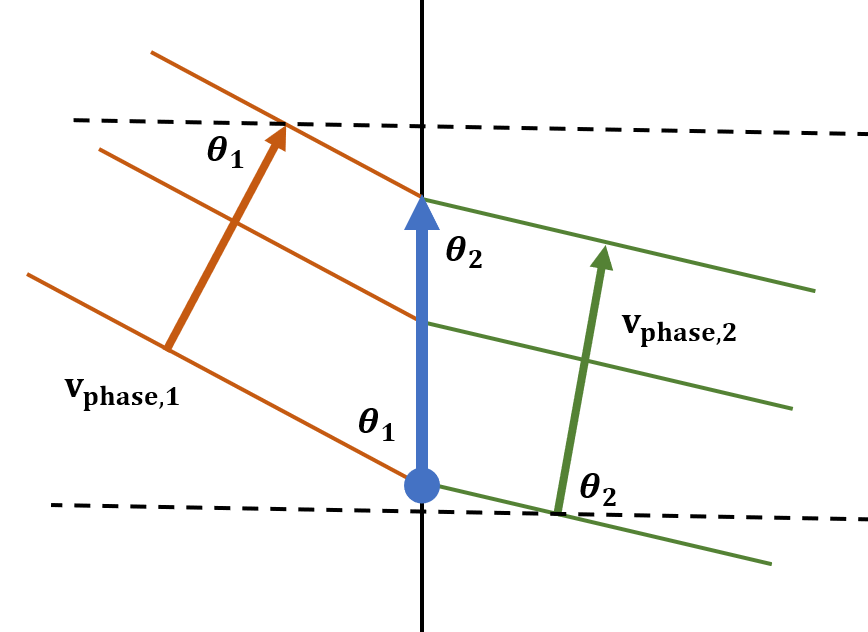
\includegraphics[width=0.6\linewidth]{Figuras/total internal reflection wave picture.png}
    \caption{Wave picture of reflection. Demanding continuity at the interface gives us Snell's Law.}
    \label{fig:total.internal.reflection.wave.picture}
\end{figure}

Look at Figure \ref{fig:total.internal.reflection.wave.picture}. One wavefront comes towards the interface with a phase velocity $v_1$ at an angle of incidence $\theta_1$, and it is refracted at $\theta_2$, with a phase velocity $v_2$. Both $v_1$ and $v_2$ are completely determined by the properties of the material, they will obey $v_i=c/n_i$, as mentioned above.

All we have left to ensure continuity at the interface is to adjust the angles $\theta_1$ and $\theta_2$. They are the angles between the plane of the interface and the planes normal to each set of wavefronts. The wavefronts must meet at a point in the interface, which moves along it at velocity $v_{node}$.

\textbf{At each side of the interface, the phase velocities must be the projection of the node velocity in the direction normal to the wavefronts}. This is a pretty straightforward consequence of demanding that the node remains at the point of ``contact'' between the wavefronts as they move along. Geometrically, this can be written as
\begin{equation}
    v_{node}=\frac{v_{\text{phase,1}}}{\sin(\theta_1)}=\frac{v_{\text{phase,2}}}{\sin(\theta_2)}.
\end{equation}
Rewrite $v_i=c/n_i$ and obtain Snell's Law
\begin{equation}
    n_1\sin(\theta_1)=n_2\sin(\theta_2).
\end{equation}

Here's something that is usually not addressed in books: why are we projecting the node velocity on the phase velocity, and not the contrary? Is not the phase velocity just the phase velocity component in the direction of the interface? \textbf{Crucially, no}. That would be the case if we wanted the node to be a \textit{shadow} of any point the wavefront, but actually we just want it to remain as a node. This is shown in Figure \ref{fig:projection.velocities.TIR}.

\begin{figure}[H]
    \centering
    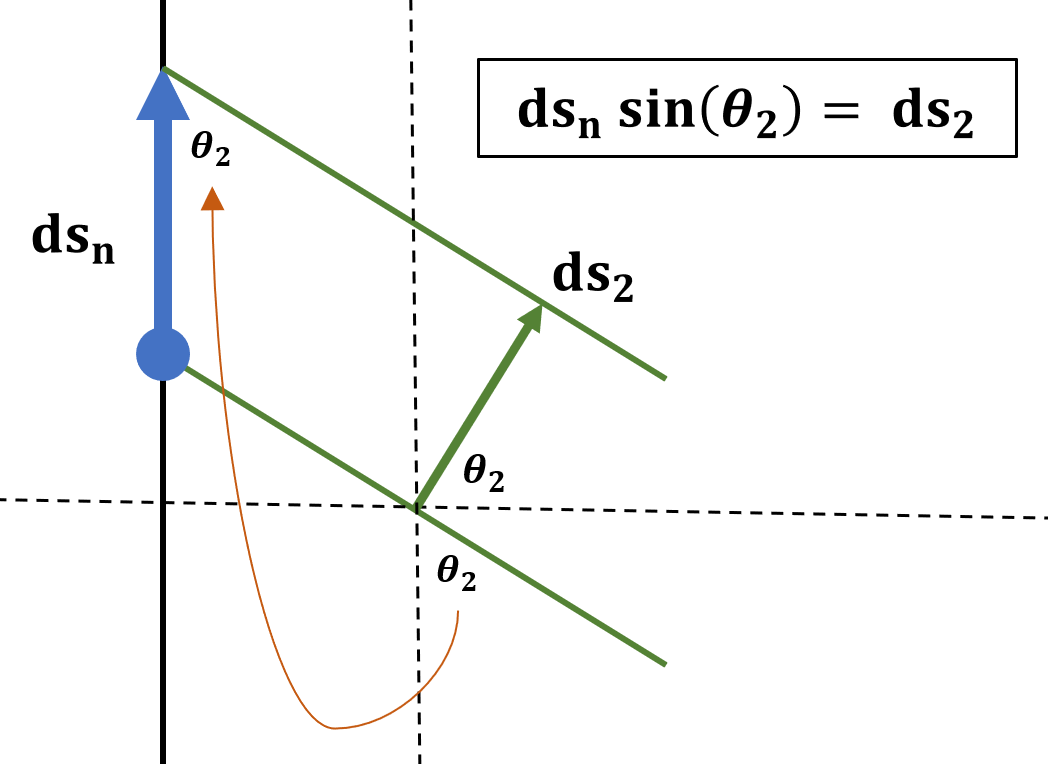
\includegraphics[width=0.6\linewidth]{Figuras/geometry wave description of TIR.png}
    \caption{A better explanation of why the phase velocities are projections of node velocity, and not the other way around.}
    \label{fig:projection.velocities.TIR}
\end{figure}

Now we should consider a few scenarios, to how this leads naturally to total internal reflection.

\subsection*{(A) Changing the incidence angle}

\textbf{As the incidence angle gets smaller}, the node velocity must increase in order to provide the appropriate contribution in the direction of the incident phase velocity. How will the phase velocity on the other side react to that? It has to point in a direction such that the projection of the node velocity in that direction is equal to $c/n_2$. As the node velocity gets higher, \textbf{it is forced to make $\theta_2$ smaller as well}.

Conversely, \textbf{as the incidence angle gets larger}, the node velocity must decrease, or else its projection in incident direction will become larger than $c/n_1$. Now that the node moves more slowly, \textbf{the refracted angle must also increase}, getting closer to becoming parallel.

From Snell's Law, we could have just noted that the sine function increases monotonically in $0<\theta<\pi/2$, but this is much more interesting.

\subsection*{(B) Changing the refractive indexes}

\textbf{If the refractive index $n_1$ is larger than $n_2$}, that means the wavefronts move slower in the incident side. Therefore, the node velocity will generally be slower than what we would get from the refracted wave at the same angle. The solution is to have the \textbf{refracted phase velocity point further away from the normal}. That way, the projection of the node velocity in the refracted direction is large enough to obey $c/n_2$. This is the fundamental condition for total internal reflection. It implies that there will be a critical angle in which $\theta_1<\pi/2$, but $\theta_2=\pi/2$.

\textbf{If the refractive index $n_1$ is smaller than $n_2$}, that means the wavefronts move faster in the incident side. Therfore, the node velocity will generally be faster than what we would get from the refracted wave at the same angle. The solution is to have the \textbf{refracted phase velocity point closer to the normal}. That way, the projection from the node velocity in the refracted direction is small enough to ``compensate'' the large node velocity and obey $c/n_2$. There will be no total internal reflection.

Mathematically, we could have just looked at Figure \ref{fig:snell.law}. It clearly shows that we only get $\theta_t=\pi/2$ when $n_1>n_2$. But now we know \textit{why} this is the case.

\begin{figure}[H]
    \centering
    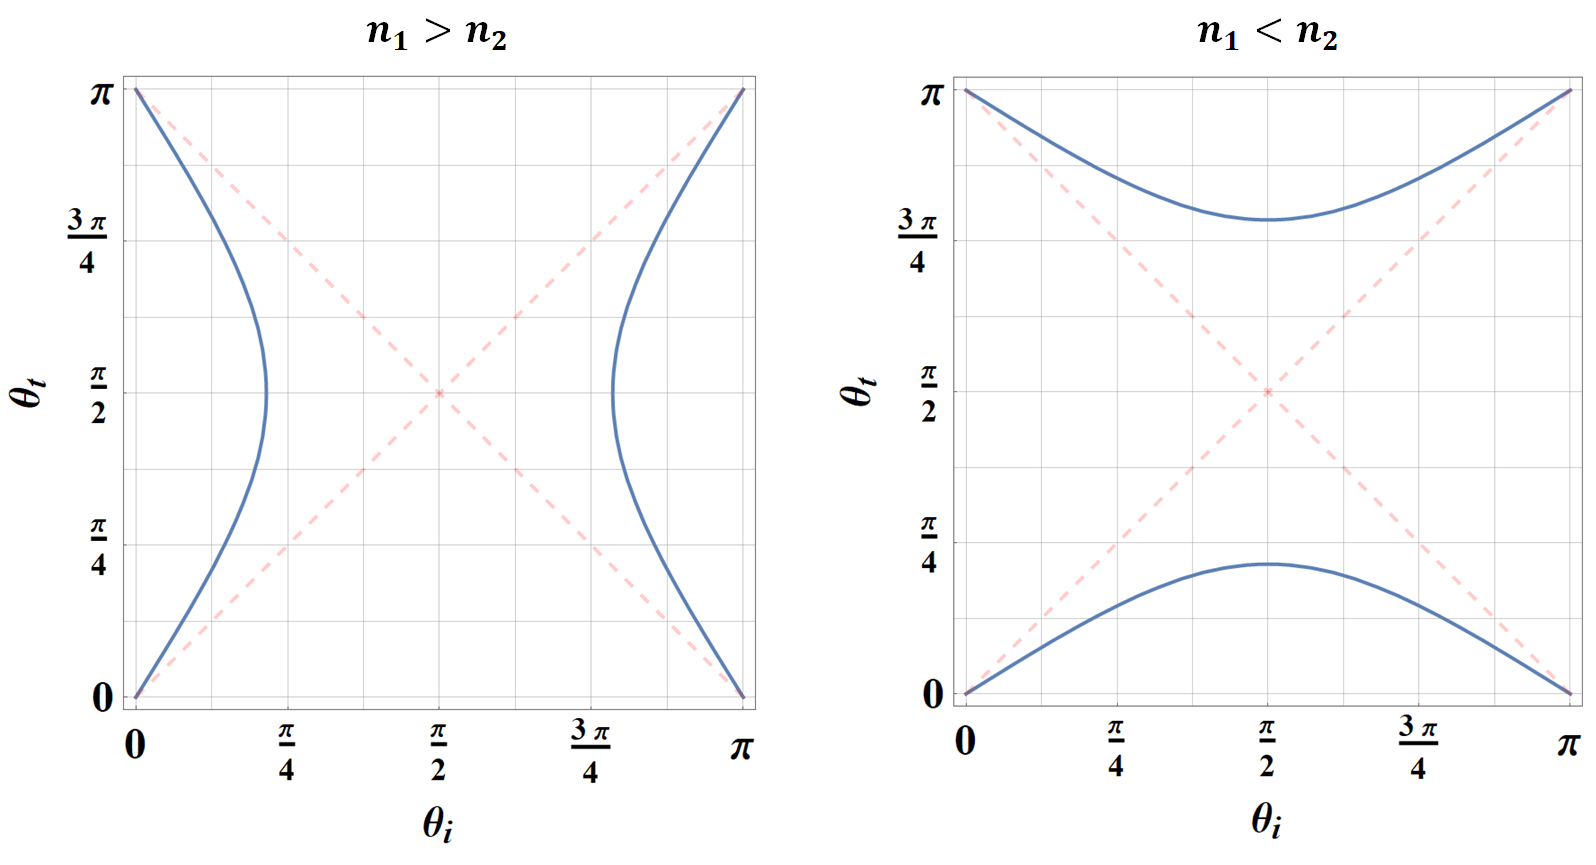
\includegraphics[width=1\linewidth]{Figuras/snell solutions.png}
    \caption{Solutions to Snell's law for $n_1>n_2$ and $n_1<n_2$. Dotted line indicates $n_1=n_2$. $n_1>n_2$ allows total internal reflection. The only physically meaningful angles are in the $0<\theta_t<\pi/2$. interval}
    \label{fig:snell.law}
\end{figure}

Clearly, when we reach the critical angle, and the refracted wave velocity is parallel to the interface, the refracted wavefronts must be perpendicular to it. What if we go beyond the critical angle?

Now the node, determined by the incident angle and velocity, is really slow. We have already done all that was possible to have the nodes meet at the interface: \textbf{the refracted wavefronts are moving too fast}. At some point, they will travel ahead of the node that created them, and meet out-oh-phase nodes in the interface, causing destructive interference. This is the physics behind the \textbf{attenuation coefficient}. Let us look at the equations to understand this effect.

\subsection*{Propagation and Attenuation Coefficients}

If the waves in Figure \ref{fig:total.internal.reflection.wave.picture} are polarized in the $x$ direction (with $+y$ pointing to the right, and $+z$ to the bottom), the (spatial parts of the) equations are given by
\begin{equation}
    \textbf{E}_1(y,z)=\hat{\textbf{x}}E_0e^{-ik_0n_1\left(z\cos\theta_1-y\sin\theta_1\right)}\;\;\;\text{and}\;\;\;\textbf{E}_2(y,z)=\tau\hat{\textbf{x}}E_0e^{-ik_0n_2\left(z\cos\theta_2-y\sin\theta_2\right)}
\end{equation}
It is easy to see that the expression for $\textbf{E}_2$ can be completely rewritten in terms of the incident angle, just by using Snell's law, as in
\begin{equation}
    \textbf{E}_2(y,z)=\tau\hat{\textbf{x}}E_0\exp\left[-ik_0n_2\left(z\sqrt{1-\frac{n_1^2}{n_2^2}\sin^2\theta_1}-y\frac{n_1}{n_2}\sin\theta_1\right)\right].
\end{equation}
At the critical angle, the term inside the square root is zero, and the transmitted field is a plane wave traveling in the $+y$ direction, parallel to the interface. On the other hand When we go beyond the critical angle $\theta_1>\sin^{-1}(n_2/n_1)$, the first term in the exponential will become imaginary: an \textbf{attenuation coefficient} will arise. This coefficient is given by
\begin{equation}
    \gamma=k_0n_2\sqrt{\frac{n_1^2}{n_2^2}\sin^2\theta_1-1},
    \label{eq:attenuation.coefficient.chap.1}
\end{equation}
Such that
\begin{equation}
    \textbf{E}_2(y,z)=\tau\hat{\textbf{x}}E_0\exp\left[-\gamma z+ik_0n_1y\sin\theta_1\right].
\end{equation}
Finally, the coefficient in the second term determines the phase change due to displacement along the direction parallel to the interface. This quantity will be defined as the \textbf{propagation coefficient} (I'll call it ``constant'' later, in the mode picture)
\begin{equation}
    \beta=k_0n_1\sin\theta_1.
\end{equation}
This coefficient is essentially the wavevector (adjusted by the refractive index) component parallel to the interface. A larger propagation constant correspond to more violent phase-oscillations. In a more general sense, we can write the transmitted field as
\begin{equation}
    \textbf{E}_2(y,z)=\tau\hat{\textbf{x}}E_0e^{-\gamma z}e^{i\beta y}.
\end{equation}

Finally, we might consider the phase introduced by reflection, simply by looking at the Fresnel Equations for the reflected field
\begin{equation}
    \frac{E_r}{E_i}=\frac{n_1\cos\theta_1-n_2\cos\theta_2}{n_1\cos\theta_1+n_2\cos\theta_2}=\abs{r}e^{i2\Phi}
\end{equation}
The take home lesson is: phase change upon reflection depends on the incidence angle. Figure \ref{fig:phase.at.TIR} provides numerical values for phase shift (note that $\phi$ is only half the phase).

\begin{figure}[H]
    \centering
    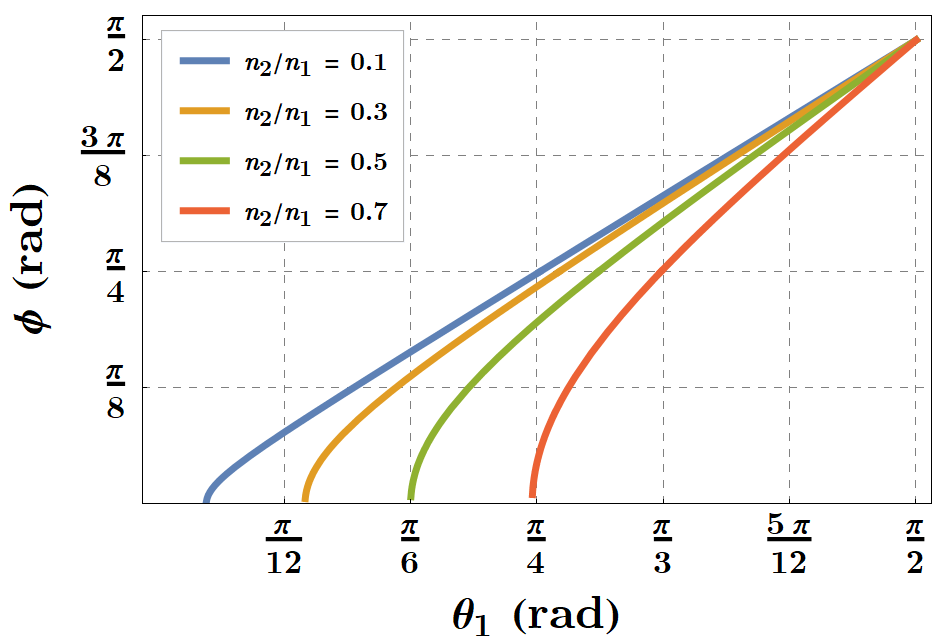
\includegraphics[width=0.8\linewidth]{Figuras/phase shift at TIR.png}
    \caption{Phase shift (half) for a TE wave as a function of the incidence angle for several refractive index ratios.}
    \label{fig:phase.at.TIR}
\end{figure}

This concludes a very intuitive discussion of how total internal reflection occurs, and how it affects the properties of waves.

\section{Modes in a planar slab waveguide}

We can describe an infinite slab waveguide by the height $h$ of its core, and the three refractive indexes of the materials that make up its core, substrate and cover. Let us consider such a waveguide, infinite in the $yz$ plane, with its height stretching along the $x$ direction. Clearly, in this picture, the TE mode means the electric field points in the $y$ direction. The refractive index of the core must be larger than the other two.

Now we derive the well known Helmholtz equation for the TE electric field. Recall the wave equation shown in the beginning of the chapter,
\begin{equation}
    \nabla^2\textbf{E}-\mu\epsilon\frac{\partial^2\textbf{E}}{\partial t^2}=0,
\end{equation}
and project it in the $y$ direction. The time derivatives will bring out a $-\omega^2$ factor, therefore
\begin{equation}
    -\mu\epsilon\frac{\partial^2E_y}{\partial t^2}=\mu\epsilon\omega^2=\frac{1}{v^2}\omega^2=\frac{n^2}{c^2}\omega^2=k_0^2n^2,
\end{equation}
and the wave equation turns into
\begin{equation}
    \nabla^2E_y+k_0^2n^2E_y=0,\;\;\;\;\Rightarrow\;\;\;\;E_y(x,z)=E_y(x)e^{-i\beta z}
\end{equation}
That "implies" symbol is not really fair, because the obvious trial solution follows from the boundary conditions, not from the PDE itself. The wave acquires a phase shift in the propagation direction, and its amplitude varies only along the confined dimension (that is, $x$). Nothing happens in the polarization direction. The trial solution will turn the Helmholtz equation into
\begin{equation}
    \frac{\partial^2 E_y}{\partial x^2}+(k_0^2n^2-\beta^2)E_y=0,
    \label{eq:helmholtz.beta}
\end{equation}
which clearly has an oscillatory solution when the term in parenthesis is positive, and an exponentially decaying one when it is negative.
\begin{itemize}
    \item In the oscillatory solution, when $\beta<k_0n$, we shall have
    \begin{equation}
        E_y(x,z)=E_0\exp(-i\beta z)\exp\left(\pm i \sqrt{k_0^2n^2-\beta^2}x\right)\;\;\;\;\kappa=\sqrt{k_0^2n^2-\beta^2}
    \end{equation}
    The transverse wavevector $\kappa$ and the propagation coefficient (longitudinal wavevector) $\beta$ are just the $x$ and $z$ components of the wavevector $k=k_0n$.
    \item In the exponential solution, we shall have an attenuation coefficient in the $x$ direction, which is identical to the one predicted in Equation \ref{eq:attenuation.coefficient.chap.1}, as it should be.
    \begin{equation}
        \gamma=\sqrt{\beta^2-k_0^2n^2}
    \end{equation}
\end{itemize}

If $\beta$ has the appropriate value to allow oscillatory solutions only inside the core of the waveguide, we should have a solution like
\begin{subequations}
    \begin{equation}
    E_y(x)=Ae^{-\gamma_cx};\;\;\;\;x>0
    \end{equation}
    \begin{equation}
    E_y(x)=B\cos(\kappa_fx)+C\sin(\kappa_fx);\;\;\;\;-h<x<0
    \end{equation}
    \begin{equation}
    E_y(x)=Ae^{-\gamma_s(x+h)};\;\;\;\;x<-h
    \end{equation}
\end{subequations}
There are four coefficients (A,B,C,D) to be found, in addition to $\gamma_c$, $\kappa_f$ and $\gamma_s$, which are all determined by $\beta$, so \textbf{five variables in total}. We will now find \textbf{four} boundary conditions, which will leave one degree of freedom, and will lead to a transcendental equation between the transverse wave-vector and the attenuation coefficients.

Imposing the boundary conditions is very tedious, but also very straight-forward, so I will skip it here for now. Essentially, just demand that $E_y$ (tangential electric field) be continuous at both the interfaces, this will give you two conditions. Next, demand that $H_z$ (tangential magnetic field) be continuous at both interfaces. It is easy to show that $H_z$ depends on the derivative of $E_y$ with respect to $x$. Finally, we will get
\begin{equation}
    \tan(h\kappa_f)=\frac{\gamma_c+\gamma_s}{\kappa_f\left[1-\frac{\gamma_c\gamma_s}{\kappa_f^2}\right]},
\end{equation}
which is the \textbf{characteristic equation for TE modes of a slab waveguide}, which yields eigenvalues $\beta_{TE}$ for allowed modes. The solution is different for TM modes.

Bottom line: infinite slab waveguides with a dense core and rarer cover/substrate will \textbf{only allow specific discrete modes to exist inside them}, and these modes will be determined by \textbf{propagation constant} $\beta$ eigenvalues, and will \textbf{obey the characteristic equation, forming a complete and orthogonal set}. Assuming, of course, that you have already chosen a specific wavelength, refractive indexes and the geometry of the waveguide (for a slab, $h$ alone will suffice).

Naturally, if you are changing the propagation coefficient while keeping the wavelength constant, then you are simply changing the allowed incidence angles (think in the ray picture). Obviously, the transverse wave vectors, which give you the mode profile, are also determined by the incidence angle. In this sense, the allowed modes in a waveguide (amplitude vs. $x$-position in $-h<x<0$) look very much like the well-known solution for a particle in a box in quantum mechanics, or for standing waves in a string.

%\todo[inline]{The book mentions that a the discrete nature of $\beta$ can be demonstrated by demanding that the accumulate phase shift (including the shift associated with reflections at both interfaces and that given by the propagation constant) be a multiple of $2\pi$. Since this formulation also yields unique solutions for $\beta$, I assume it must be equivalent to the formulation I just demonstrated using Maxwell's equations with the appropriate boundary conditions. But I still need to demonstrate this equivalence. Come to think of it, the phase shifts themselves are given by Fresnel equations, which in turn are also derived from Maxwell's equations with the same boundary conditions. So I guess it is not even worth checking.}

\section{Propagation parameters}

How many modes are there in a waveguide for a given wavelength and geometry? According to the characteristic equation, we know that these modes correspond to points where
\begin{equation}
    \tan(h\kappa_f)=\frac{\gamma_c+\gamma_s}{\kappa_f\left[1-\frac{\gamma_c\gamma_s}{\kappa_f^2}\right]}.
\end{equation}
So that if we think in terms of the transverse wavevector, and consider that the \textit{tangent} function repeats itself in intervals of $\pi$, then clearly there are more modes when $h\kappa_f$ gets larger.

Mathematically, consider the following: $\tan(h\kappa_f)$ goes from $-\infty$ to $\infty$ in each and every one of its periods. Clearly, if $\kappa$ is allowed to grow, then more periods are ``unlocked'', and in every period there will certainly exist at least one crossing of the tangent function with the quotient on the right side of the characteristic equation.

Physically, in the ray picture, whichever factor we increase in $h\kappa_f$ is equivalent to allowing more incidence angles above critical. In the wave picture, there are more ways for the wave to travel back and forth between the interfaces and maintain a net phase shift that is a multiple of $2\pi$, as in:
\begin{equation}
    2k_0n_1h\cos\theta-2\Phi_1-2\Phi_2=2\pi N.
\end{equation}
We might say that the number $m$ of modes allowed in the waveguide is proportional to how many times $h\kappa_f$ can be bigger than $\pi$
\begin{equation}
    m=\text{Int}\left(\frac{h\kappa_{max}}{\pi}\right).
\end{equation}
But the transverse wavevector will be largest when the wavevector in the core is closest to the critical angle. In that case, the \textbf{transverse} component will be given by
\begin{equation}
    \kappa_{max}\approx k_0n_1\cos\theta_1=k_0n_1\sqrt{1-\frac{n_2}{n_1}}=k_0\sqrt{n_1^2-n_2^2},
\end{equation}
therefore
\begin{equation}
    m=\text{Int}\left(\frac{hk_0\sqrt{n_1^2-n_2^2}}{\pi}\right).
\end{equation}
Here, we are assuming a symmetrical waveguide, so let us call $n_2$ the \textit{cladding} refractive index. Now it is only natural to define a \textbf{normalized frequency} (measured in radians)
\begin{equation}
    \boxed{V=\frac{2\pi h}{\lambda}\sqrt{n_1^2-n_2^2}}
\end{equation}
The normalized frequency tells us approximately how many modes are allowed in our waveguide. Just divide it by $\pi$, and you will know how many full periods the tangent function in the characteristic equation has covered.

It makes sense that thicker waveguides should accommodate more modes for a fixed wavelength: there are more ways to fit the waves there so that total phase shift is $2\pi$ between the interfaces. The same is true for vibration modes on a string with fixed ends. It also makes sense that there should be some dependence on the refractive indexes, for they will give you the phase shift upon reflection at the interfaces.

We now turn to another very important parameter: the \textbf{effective refractive index}, which is widely used to characterize modes in simulation software. The effective index is defined as
\begin{equation}
    \boxed{n_{eff}=\frac{\beta}{k_0},}
\end{equation}
We know that $\beta$ is the longitudinal component of the wavevector, and that the wavevector inside a medium differs from its magnitude in a vacuum by a factor $n$. So all that is left when we divide the propagation constant $\beta$ by $k_0$ is information concerning how the material changes the wavevector, and about the incidence angle associated with the specific mode.

Perhaps the physical significance of $n_{eff}$ becomes clearer when it is written as in $\beta=n_{eff}k_0$: the \textbf{effective refractive index tells you how the phase-shift per unit length in the guided mode compares to the phase-shift per unit length in a vacuum}. If you are comfortable with characterizing modes via propagation constants, you only have to take one extra step: a number which tells you how different this propagation constant is from its equivalent in a vacuum (where there is no medium and no confinement).

Here is one question which encompasses almost all that we have covered so far: \textbf{why would you expect higher-order modes to have a lower effective refractive index?}

\noindent \textit{Answer}.: Think about modes on a string. Higher order modes can fit more wavelengths in the same string. In a slab waveguide, if the height is held fixed, the only way to fit more modes is for the transverse wavevector to be larger (so that phase shifts more quickly along the height!). When you increase the transverse wavevector, you inevitably decrease its longitudinal counterpart. For that reason, higher order modes will have lower effective index.

Most textbooks also discuss the \textbf{numerical aperture} as a way to characterize waveguides. We know that guided waves can only occur when the incidence angle at the waveguide's interface is equal or higher than critical, so as to allow total internal reflection. The question is: at what angles can you introduce a ray of light from air and into the core of the waveguide so that it can be refracted in a direction such that it strikes the core-cladding interface at the appropriate angle interval. The sine of the highest of these allowed angles will define the \textbf{numerical aperture}, and the set of allowed angles will define \textit{the acceptance angle}.

\section{Cut-off conditions}

Cut-off conditions for the slab waveguide do not translate very well to different geometries. They can, however, help us get a much better understanding of the role played by the normalized parameters. From the Helmholtz equations shown in \ref{eq:helmholtz.beta}, we know that guided modes (corresponding to solutions which are oscillatory in the core and exponentially decaying in the cladding) must satisfy
\begin{equation}
    k_0n_{\text{cladding}}\le \beta \le k_0n_{\text{core}}\;\;\;\;\Rightarrow\;\;\;\;n_{\text{cladding}}\le n_{\text{eff}}\le n_{\text{core}},
\end{equation}
where I am assuming a symmetric waveguide. The effective refractive index also tells you, by a simple comparison to known data, which modes can be guided. Now it is only natural to define another parameter, \textit{the normalized effective index} $b$, through some manipulations of the previous inequality. Since $n$ is always greater than $1$, we can square the inequality to get
\begin{subequations}
    \begin{equation}
        n^2_{\text{cladding}}\le n^2_{\text{eff}}\le n^2_{\text{core}},
    \end{equation}
    \begin{equation}
        0\le n^2_{\text{eff}}-n^2_{\text{cladding}}\le n^2_{\text{core}}-n^2_{\text{cladding}},
    \end{equation}
    \begin{equation}
        0\le\left(\frac{n^2_{eff}-n^2_{cladding}}{n^2_{core}-n^2_{cladding}}\right)\le 1,\;\;\;\;\;\;b\equiv\frac{n^2_{eff}-n^2_{cladding}}{n^2_{core}-n^2_{cladding}}.
    \end{equation}
\end{subequations}
We have now obtained a simple, dimensionless parameter which predicts whether a mode will be guided or not. How does this fit into our characteristic equation? We noted that another way to express the eigenvalue equation for TE modes is
\begin{equation}
    2k_0n_1h\cos\theta-2\Phi_1-2\Phi_2=2\pi N.
\end{equation}
We may use the Fresnel equations to express the phase-shifts at the interfaces. Considering a symmetric waveguide, $n_1=n_{core}$, $n_2=n_{cladding}$, so that the phase-shift is equal in both interfaces, we can be write the eigenvalue equation as
\begin{subequations}
\begin{equation}
    2k_0n_1h\cos\theta-4\tan^{-1}\left[\frac{\sqrt{n_1^2\sin^2\theta_1-n_2^2}}{n_1\cos\theta_1}\right]=2\pi N,
\end{equation}
\begin{equation}
    k_0h\sqrt{n_1^2(1-\sin^2\theta)}-2\tan^{-1}\left[\frac{\sqrt{n_{eff}^2-n_2^2}}{n_1\sqrt{1-\sin^2\theta_1}}\right]=\pi N
\end{equation}
\begin{equation}
    k_0h\sqrt{n_1^2-n^2_{eff}}-2\tan^{-1}\left[\sqrt{\frac{n_{eff}^2-n_2^2}{n_1^2-n^2_{eff}}}\right]=\pi N
\end{equation}
\begin{equation}
    \frac{V}{\sqrt{n_1^2-n_2^2}}\sqrt{n_1^2-n^2_{eff}}-2\tan^{-1}\left[\sqrt{\frac{n_{eff}^2-n_2^2}{n_1^2-n^2_{2}}\frac{n_1^2-n_2^2}{n_1^2-n_{eff}^2}}\right]=\pi N
\end{equation}
\begin{equation}
    V\sqrt{1-b}-2\tan^{-1}\left[\sqrt{b\left(\frac{1}{1-b}\right)}\right]=\pi N
\end{equation}
\begin{equation}
    V\sqrt{1-b}=N\pi+2\tan^{-1}\sqrt{\frac{b}{1-b}}
\end{equation}
\end{subequations}

Now we can do everything with a few dimensionless quantities! When interpreting the following numerical results, keep a few things in mind:
\begin{itemize}
    \item The normalized frequency contains the $h/\lambda$ ratio and the $\sqrt{n_1^2-n_2^2}$ difference between clad and core indexes.
    \item The normalized effective index is a dimensionless indicator of whether a mode is guided or not. A guided mode must have $0\le b\le 1$.
    \item $V$ and $b$ are not to be thought of as functions of each other: they are both functions of multiple other parameters. It is useful, however, to think of $V$ as the variable over which we have some control. As it changes, the characteristic equation will allow different values for $b$ and order $N$, each of which correspond to a mode.
    \item Multiple values of $b$ can correspond to modes of the same order $N$. In general, each normalized frequency will have, at most, one solution for each mode order. The normalized frequency at which a given mode ceases to exist is called a \textit{cutt-off} frequency.
\end{itemize}

Figure \ref{fig:characteric.equation} illustrate the points above. If your slab geometry, input wavelength and refractive indexes are chosen, a set of modes corresponding to $b$-values greater than zero will be guided in your waveguide. As $V$ increases, more modes are allowed. The frequency at which a given mode dies is called the \textit{cut-off} frequency.

\begin{figure}[h]
    \centering
    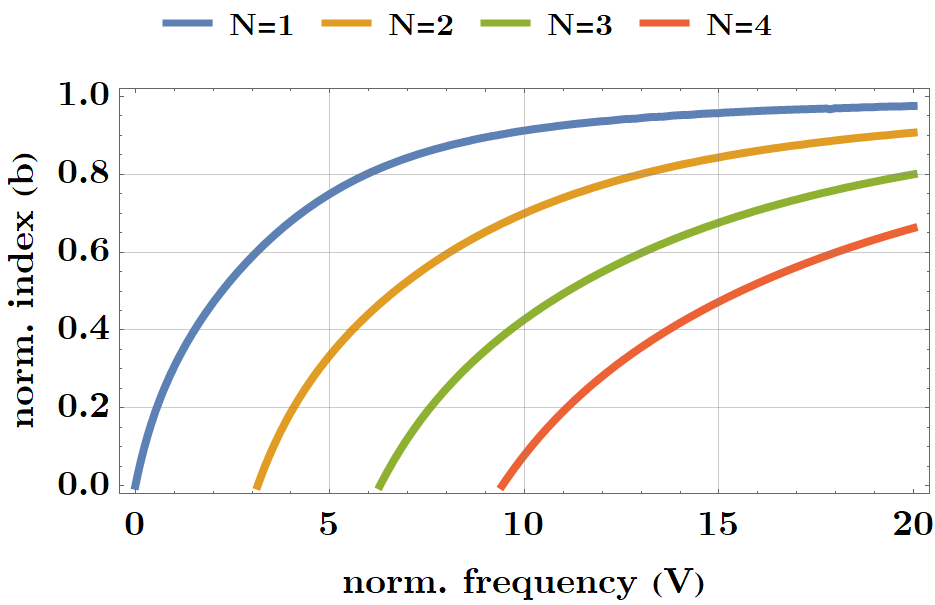
\includegraphics[width=0.8\linewidth]{Figuras/characteristic equation.png}
    \caption{Solutions for the characteristic equation in terms of normalized parameters. If an asymmetric waveguide were employed, small changes would be observed for each mode. As $V$ increases, more modes are allowed.}
    \label{fig:characteric.equation}
\end{figure}

\hrulefill

This concludes the review of basic concepts needed for a theory of optical waveguides. Analytical solutions for mode eigenvalues, like the ones we derived here, are generally not available for waveguides actually suited for practical applications, and so these must be handled with numerical methods and reasonable approximations. I will skip taking notes on the circular waveguide, which differs from the slab waveguide in predictable manners (circular boundary conditions lead to Bessel solutions), and go straight to the rectangular waveguide, which is of greater interest to integrated optics.

\hrulefill
\newpage
\section{Rectangular Waveguides}

Next, we consider the waveguide illustrated in Figure \ref{fig:rec.waveguide}. \textbf{The treatment of the rectangular waveguide is mostly a matter of choosing appropriate approximations}.  In this section we will consider two of them: Macartilli's method, and the effective index method.

A quick word on notation: although there are no pure TE or TM modes in a rectangular waveguide, they can still be strongly polarized in one direction, and thus be labeled as \textit{quasi-TM} and \textit{quasi-TE}. A mode displaying an electric field strongly polarized along the $x$ direction can be characterized by two indexes $p$ and $q$, and we refer to which by $E^x_{pq}$ or, conversely, $E^y_{pq}$.

\subsection{Marcatilli's method}

The first approximation which we will consider is that the field is negligible in the shaded regions in Figure \ref{fig:rec.waveguide}, the coupling of the $x$ and $y$ solutions makes it so that separation of variables becomes unattainable in these regions. This complication should be obvious if you begin to consider what it would be like to impose the appropriate boundary conditions in the corners of the rectangle. When modes are very far from cut-off (think of a very high $b$ in Figure \ref{fig:characteric.equation}), the fields are well confined in the core, and this approximation becomes very reasonable.

\begin{figure}[h]
    \centering
    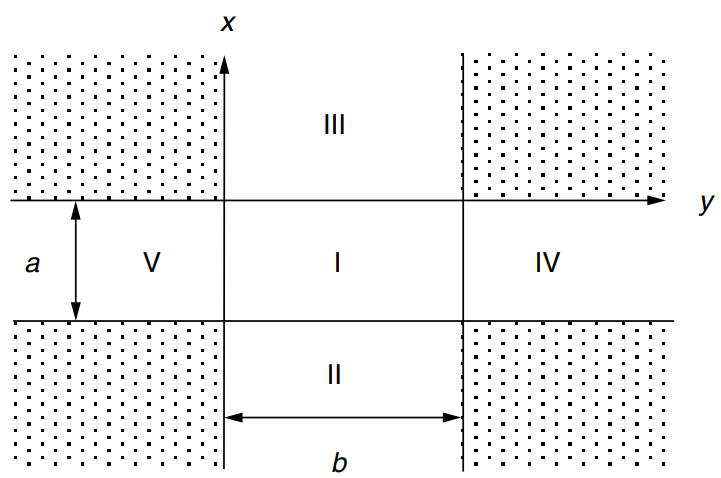
\includegraphics[width=0.6\linewidth]{Figuras/three dimensional rectangular waveguide.png}
    \caption{Three dimensional rectangular waveguide}
    \label{fig:rec.waveguide}
\end{figure}

It should be obvious that the wave equation will now look like
\begin{equation}
    \nabla\cdot\textbf{E}-\mu\epsilon\frac{\partial^2 E}{\partial t^2}=0\;\;\;\Rightarrow\;\;\;\frac{\partial^2 E}{\partial x^2}+\frac{\partial^2 E}{\partial y^2}+(k_0^2n^2-\beta^2)E=0.
\end{equation}
Where we are simply, and reasonably, assuming that the solution is of the form $E=E(x,y)e^{-i\beta z}$. When a separation of variables is proposed, this equation will become
\begin{equation}
    \frac{\ddot{X}}{X}+\frac{\ddot{Y}}{Y}+k_0^2n^2(x,y)-\beta^2=0.
\end{equation}
Clearly, we can introduce separation constants which have clear physical meaning. We want the solution to be oscillatory in the core, that is,
\begin{equation}
    X(x)=A\cos(\kappa_xx+\phi_x)\;\;\;\text{and}\;\;\;Y(y)=B\cos(\kappa_yy+\phi_y).
\end{equation}
The wave equation demands that
\begin{equation}
    \boxed{k_0^2n_1^2=\beta^2+\kappa_x^2+\kappa_y^2.}
\end{equation}
What happens outside the core? Now we have to worry about two things:
\begin{enumerate}
    \item All field components must vanish far away from the core, so at least one of the separated solutions must decay exponentially.
    \item The transverse fields ($x$ and $y$) must be continuous across the dielectric interfaces.
\end{enumerate}
The only way for these concerns to be met is to make the y dependent field solution identical along the $x$ axis, and the $x$ dependent field solution identical along the $y$ axis (by identical I mean ``of the same form''). Therefore, in Figure \ref{fig:rec.waveguide}, $Y(y)$ will be sinusoidal in regions I, II and III, and exponentially decaying in regions IV and V; On the other hand, $X(x)$ will be sinusoidal in regions I, IV and V, and exponentially decaying in regions II and III.

Note that if $Y(y)$ were, for instance, sinusoidal in I and exponential in II or III, it would be absurd to require continuity at every point in the interface, since $y$ is confined to $0\le y \le b$ in this regions. Note also that if $X(x)$ were not exponential in regions II and III, there would be no way to ensure that $X(x)Y(x)$ decays, for the same reason as before: $y$ is limited.

We already know what the sinusoidal solutions look like, and what conditions the wavevectors $\kappa_i$ obey. What conditions do the attenuation factors in the exponential decaying functions obey? Just go back to the separated wave equation
\begin{equation}
    \frac{\ddot{X}}{X}+\frac{\ddot{Y}}{Y}+k_0^2n^2(x,y)-\beta^2=0.
\end{equation}
Consider region III, for instance. The second derivative in $y$ will clearly spit out a $-\kappa^2_y$, thus
\begin{equation}
    \frac{\ddot{X}}{X}=\kappa^2_y-k_0^2n^2_3+\beta^2=0
\end{equation}
The quadratic sum of $\beta$ and $\kappa_y$ yields the core wave-vector $k_0n_1$ and $\kappa_x$, so
\begin{equation}
    \frac{\ddot{X}}{X}=-k_0^2n^2_3+k_0^2n^2_1-\kappa_x^2\;\;\;\Rightarrow\;\;\; X(x)=\exp(-\gamma_3x)\;\;\;\text{where}\;\;\;\gamma_3=\sqrt{k_0^2(n_1^2-n_3^2)-\kappa_x}.
\end{equation}
This demonstration provides a general form for the attenuation coefficients, only the refractive index for the specific region and the transverse wavevector must be adjusted.

Notice that $X(x)$ has the same \textbf{form} that you expect from a slab waveguide, infinite in $y$ and $z$; also, $Y(y)$ has the same \textbf{form} that you would expect from a slab waveguide, infinite in $x$ and $z$. In other words, this approximation leads to a rectangular waveguide mode composed of the product of two orthogonal spatial modes. The solutions are coupled through their connection with a single eigenvalue $\beta$ and the core wavevector $k_0n_1$.

Once the appropriate boundary conditions are imposed, once again in very good analogy to the slab case, the following characteristic equations will appear for $\kappa_x$ and $\kappa_y$ in the $E^x_{pq}$ case
\begin{equation}
    \tan(\kappa_yL_y)=\frac{\kappa_y(\gamma_4+\gamma_5)}{\kappa_y^2-\gamma_4\gamma_5}\;\;\;\text{and}\;\;\;\tan(\kappa_xL_x)=n_1^2\frac{\kappa_x(n_2^2\gamma_3+n_3^2\gamma_2)}{n_2^2n_3^2\kappa_x^2-n_1^2\gamma_2\gamma_3},
\end{equation}
the existence of two characteristic equations clearly indicated why we use two indexes to specify a mode. And the phases included in the general solutions are given by
\begin{equation}
    \tan(\phi_x)=-\frac{n_3^2}{n_1^2}\frac{\kappa_x}{\gamma_3}\;\;\;\text{and}\;\;\;\tan(\phi_y)=-\frac{\gamma_5}{\kappa_y}.
\end{equation}
And the normalized frequency for the rectangular waveguide is defined as
\begin{equation}
    V\equiv k_0\frac{L}{2}\sqrt{n_1^2-n_2^2},
\end{equation}
where $L$ is the smallest dimension of the waveguide and $n_2$ is the refractive index closest to the core value. These results, the latter defined and the former derived via boundary conditions, should be enough for an analysis of rectangular waveguides using the Marcatilli method. I will not plot the expected appearance of the modes, for they should be fairly obvious from the mathematical expression. I will also skip any further discussion about the effectiveness of the method in different regimes.

\subsection{Effective index method}

The effective index method is very simple. First, the rectangular dielectric waveguide is reduced to a slab waveguide, in which the light is confined in a single direction. The slab problem is then solved exactly, and the effective indexes $n_{eff}$ for the guided modes are found. Next, a second slab is considered, in which the light is confined in the direction transverse to the previous, and the refractive index of the core is taken as $n_{eff}$. Finally, this last slab problem is solved exactly, yielding approximate results for the modes of the rectangular waveguide.

\begin{figure}[h]
    \centering
    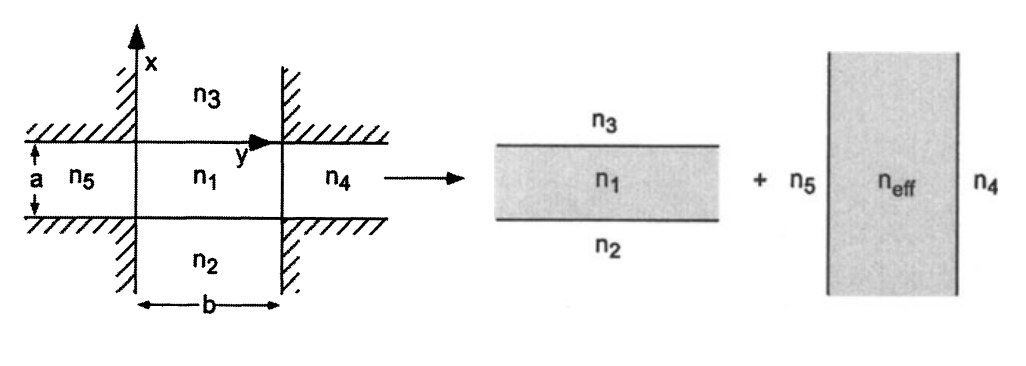
\includegraphics[width=0.8\linewidth]{Figuras/effective index method.png}
    \caption{Diagram for the effective index method.}
    \label{fig:effective.index.method}
\end{figure}

Mathematically, the method begins with the wave equation
\begin{equation}
    \frac{\partial^2E(x,y)}{\partial x^2}+\frac{\partial^2E(x,y)}{\partial y^2}+(k_0^2n^2-\beta^2)=0,
\end{equation}
and the assumption that the solution can be separated, as in $E(x,y)=\Theta(x,y)\Phi(y)$, so the equation becomes
\begin{equation}
    \Phi\frac{\partial^2\Theta}{\partial x^2}+2\frac{\partial\Theta}{\partial y}\frac{\partial\Phi}{\partial y}+\Theta\frac{\partial^2\Phi}{\partial y^2}+\Phi\frac{\partial^2\Theta}{\partial y^2}+(k_0n^2-\beta^2)\Theta\Phi=0
\end{equation}
Dividing by the product $\Theta(x,y)\Phi(y)$, we get
\begin{equation}
    \frac{1}{\Theta}\frac{\partial^2\Theta}{\partial x^2}+2\frac{1}{\Theta\Phi}\frac{\partial\Theta}{\partial y}\frac{\partial\Phi}{\partial y}+\frac{1}{\Phi}\frac{\partial^2\Phi}{\partial y^2}+\frac{1}{\Theta}\frac{\partial^2\Theta}{\partial y^2}+(k_0n^2-\beta^2)=0,
    \label{eq:intermed.EIM}
\end{equation}
now comes the first approximation, we assume that the $\Theta(x,y)$ has a very slow variation with respect to $y$, so we can neglect the second and fourth terms in Equation \ref{eq:intermed.EIM}, which gives us
\begin{equation}
    \frac{1}{\Theta}\frac{\partial^2\Theta}{\partial x^2}+\frac{1}{\Phi}\frac{\partial^2\Phi}{\partial y^2}+(k_0n^2-\beta^2)=0,
\end{equation}
Now we add a separation constant $A$, in order to get two equations
\begin{equation}
    \frac{1}{\Theta}\frac{\partial^2\Theta}{\partial x^2}+(k_0n^2-A^2)=0\;\;\;\;\text{and}\;\;\;\;\frac{1}{\Phi}\frac{\partial^2\Phi}{\partial y^2}+(A^2-\beta^2)=0,
\end{equation}
This is a brilliant solution. Notice that $\beta$ \textit{is} the rectangular waveguide's mode eigenvalue. By solving the first equation exactly, we can write $A=k_0n_{eff}$ to find the effective index of the first slab. In the second equation, the same constant $A$ appears as the core refractive index, and the equation can be solve to find the rectangular waveguide mode eigenvalues $\beta$, as illustrated in Figure \ref{fig:effective.index.method}.

\hrulefill

Further understanding of the limitations and applications of these methods is best acquired through numerical simulations, so I will stop the notes here.

\hrulefill
\newpage
\section{Dispersion in Waveguides}

\noindent Dispersion is an extremely important concept for nonlinear optics. The efficiency of nonlinear optical processes requires the fulfillment of specific phase matching conditions. In most cases, achieving phase matching is synonymous to compensating or engineering dispersion. Before going through this chapter, consider the following statements:
\begin{itemize}
    \item Every light signal has some spectral width.
    \item The refractive index always has some spectral dependence.
    \item If $n$ had no spectral dependence, then a plot of wavenumber vs. frequency would always be a straight line with slope 1/c.
    \item The wavenumber vs. frequency relation (\textit{dispersion relation}) is given by $k=n(\omega)\omega/c$, which can have a non-zero second derivative of $k$ with respect to $\omega$.
    \item If there were no dispersion, there would always be phase matching. This is the case, for instance, of Self Phase Modulation.
\end{itemize}
%
\textbf{In short, (material) dispersion is the fact that materials respond differently to different frequencies, and optical signals have multiple frequencies, so instead of halving the frequency every time the wavelength is doubled, you will have something else done. }This is equivalent to saying that the second derivative of $k$ with respect to $\omega$ is non-zero.

\subsection{Phase velocity and group velocity}

Consider a wave propagating in the $z$ direction. If I choose a point on the crest of such a wave, at what rate must it move to remain there? The answer is: at a rate equal to the \textbf{phase velocity}, which is the rate at which the phase fronts propagate in space, as is shown by
\begin{subequations}
\begin{equation}
    u(t)=\exp\left[-i(kz-\omega t)\right]\;\;\;\Rightarrow\;\;\;\Phi(x,t)=-i(kz-\omega t)
\end{equation}
\begin{equation}
    \Phi(x,t)=\text{cte}\;\;\;\Rightarrow\;\;\;z=\frac{\omega}{k}t\;\;\;\Rightarrow\;\;\;\boxed{v_p=\frac{dz}{dt}=\frac{\omega}{k}}
\end{equation}
\end{subequations}
The expression is very intuitive: $\omega$ will tell you how much the phase will shift for each unit of time, and dividing by $k$ will tell you how much you have to move through space in order to match this shift in phase, thus keeping $\Phi(x,t)$ constant. Things get a lot less intuitive when we start mixing multiple frequency components.

\subsubsection*{Group velocity}

A simple harmonic wave cannot carry information, since it is the same all throughout space and time. In order to carry information, some modulation is required. Modulation can be achieved, for instance, by a superposition of multiple frequencies spread around a so-called \textit{carrier frequency}, forming a beat. Using a few trigonometric identities, we can show that
\begin{align*}
    u&=u_0e^{i[(k_c+\Delta k)z-(\omega_c+\Delta\omega)t]}+u_0e^{i[(k_c-\Delta k)z-(\omega_c-\Delta\omega)t]}\\
    &=2u_0e^{i[k_cz-\omega t]}\cos(\Delta kz-\Delta\omega t)
\end{align*}

So by adding similar high-frequency signals, which differ from a central ``carrier'' only by small amounts, we can get an signal whose frequency is equal to those small amounts acting as an envelope around the \textit{carrier} frequency, thereby encoding a low-frequency signal traveling at the\textbf{ group velocity} on a sum of high-frequency waves. This process is shown in Figure \ref{fig:wave.packet}.

\begin{figure}[h]
    \centering
    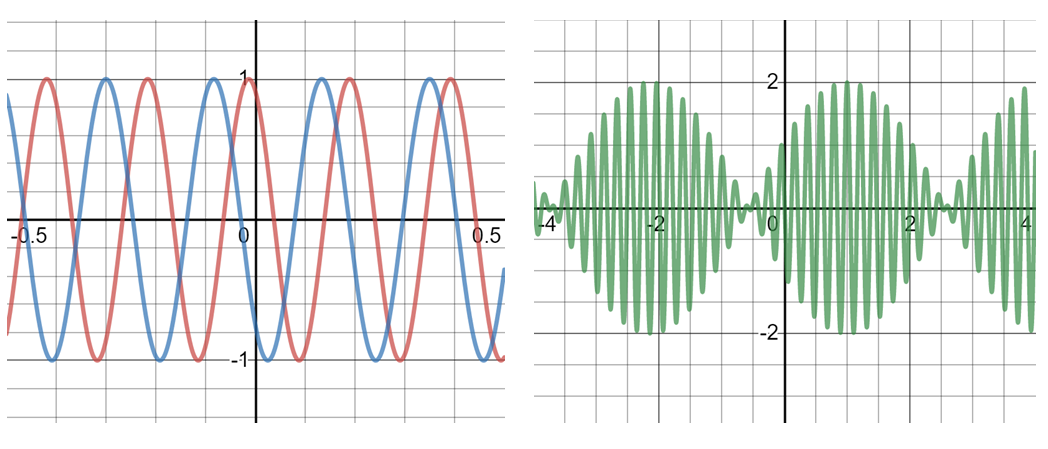
\includegraphics[width=0.45\linewidth]{Figuras/wave packet (1).png}
    \caption{Two waves, whose frequencies differs by $\Delta\omega$, and their sum.}
    \label{fig:wave.packet}
\end{figure}

I will not concern myself with \textit{why} information and energy are coupled to group velocity. For now, I will just note that it is sometimes necessary, inevitable and/or convenient to have a signal travel at the group velocity defined by a pulse of waves with different frequencies, centered around a carrier.

The important question is how to calculate the group velocity. In the case I showed above, we could clearly write
\begin{equation}
    v_g=\frac{\Delta\omega}{\Delta k}\;\;\;\xRightarrow{\Delta\rightarrow 0}\;\;\;v_g=\frac{d\omega}{dk}.
\end{equation}
Therefore,
\begin{equation}
    v_p=\frac{c}{n}=\frac{\omega}{2\pi}\lambda=\frac{\omega}{k}\;\;\;\Rightarrow\;\;\; v_g=\frac{d\omega}{dk}=\frac{d}{dk}\left(\frac{ck}{n}\right)=\frac{c}{n}-\frac{kc}{n^2}\left(\frac{dn}{dk}\right)
\end{equation}
The last derivative is the ``dispersion'', it tells you how the index of refraction changes with wavelength. In the case of \textit{regular dispersion}, the derivative is positive and group velocity is lower than phase velocity, in the case of \textit{anomalous dispersion}, the derivative is negative and group velocity is higher than phase velocity. In a vacuum, where there is no dispersion, phase velocity and group velocity are the same.

Let us try to make sense of this result. What does the group velocity has to do with how the frequency changes with wavenumber?

\begin{figure}[h]
    \centering
    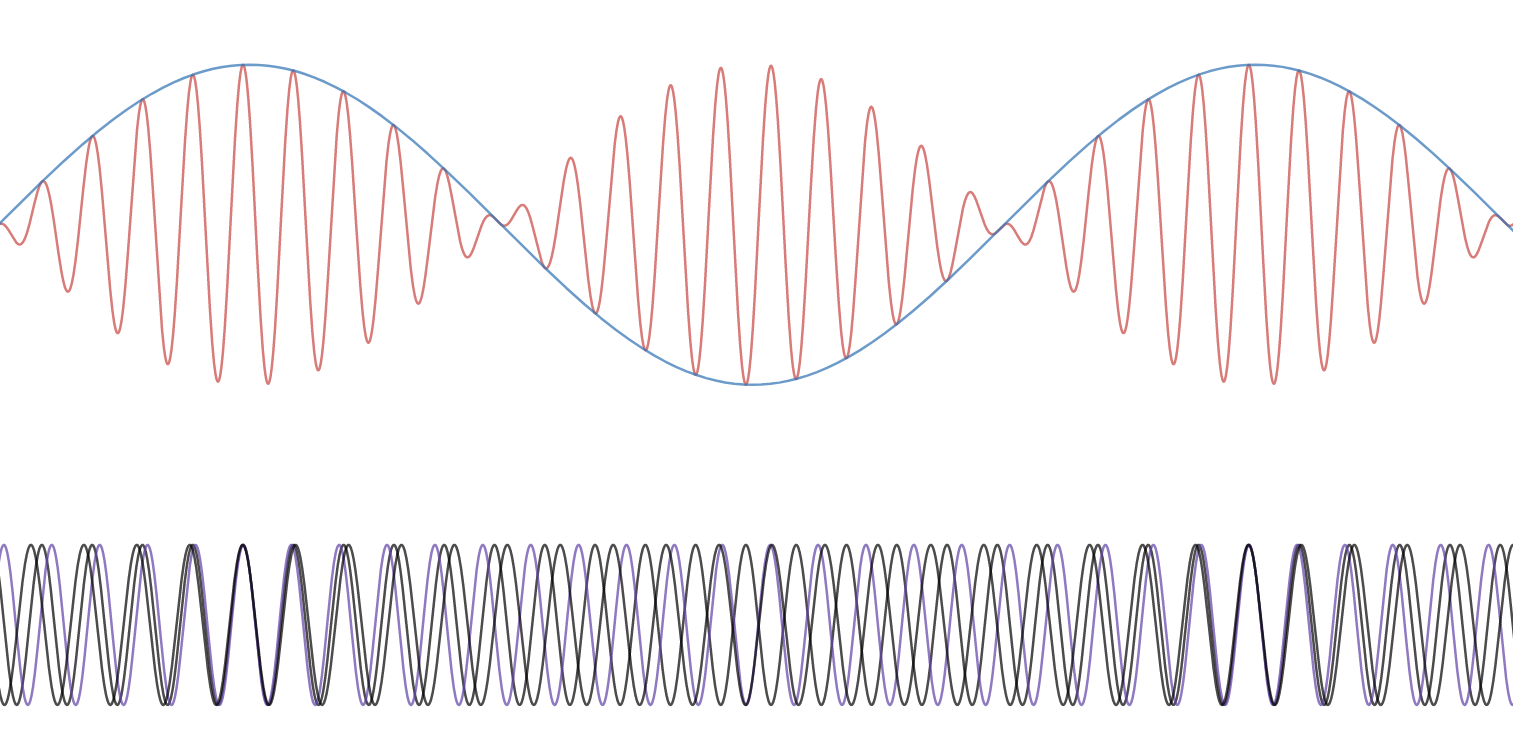
\includegraphics[width=\linewidth]{Figuras/group velocity sum.png}
    \caption{The sum of two adjacent frequencies results in a wave-packet traveling at the group velocity.}
    \label{fig:group.velocity.sum}
\end{figure}

As we have seen, group velocity is associated with an envelope which results from the sum of multiple frequencies. The positions of the peaks and nodes of the envelope are determined by the positions at which the two frequencies interfere constructively and destructively. So if you choose a point in the envelope, it corresponds to a specific combination of phases in the ``sources'', if the phase velocities of the two waves are the same, then the chose point in the envelope will move at the phase velocity, this is clear if we write
\begin{equation}
    v_g=\frac{\Delta\omega}{\Delta k}=\frac{\omega_2-\omega_1}{k_2-k_1}=\frac{(k_2-k_1)c}{k_2-k_1}=c
\end{equation}

Now, if we add dispersion to the picture, than by changing the frequency around the ``carrier'', we are changing the phase velocity in some strange manner, and any specific phase front in the envelope will move at some other speed.

Now let us look at a more general situation. What if I have a sum of multiple frequency components? Why do the frequencies have to be close to the carrier? First, write the pulse as a superposition of multiple frequency components, as in
\begin{equation}
    \psi(x,t)=\int dk\;A(k)e^{i(kx-\omega(k)t)}\;\;\;\Rightarrow\;\;\;\psi(x,0)=\int dk\;A(k)e^{ikx},
\end{equation}
and rewrite the dispersion relation in the exponent with a Taylor series around the carrier
\begin{equation}
    \psi(x,t)=\int dk\;A(k)e^{ikx}\exp it\left[\omega(k_c)+\frac{d\omega}{dk}\Biggr|_{k_c}(k-k_c)+O(k^2)\right].
\end{equation}
Now, if the spectrum of the signal is somewhat peaked around the carrier, then the contributions from terms very far from the carrier is negligible, which is why it makes sense to write the Taylor series around $k_c$. If we take the non-$k$ dependent terms away from the integral and write them as a single phase, we get
\begin{equation}
    \psi(x,t)=e^{i\Phi}\int dk\;A(k)\exp{ik\left(x-\frac{d\omega}{dk}\Biggr|_{k_c}t\right)},
\end{equation}
which, by comparison to the packet at $\psi(x,0)$, tells us that
\begin{equation}
    \abs{\psi(x,t)}=\abs{\psi\left(\left[x-\frac{d\omega}{dk}\Biggr|_{k_c}t\right],0\right)}
\end{equation}
which once again provides a better explanation for the group velocity formula: the magnitude of the wave packet at any position and time is equal to the magnitude $t=0$ at a position displaced by $\frac{d\omega}{dk}t$. This derivation also eliminates some ambiguity in the previous result: the group velocity corresponds to the derivative evaluated \textit{at the carrier frequency}, not at the frequency of the envelope itself.

This is enough discussion about the group velocity, let us look at dispersion phenomena, both in general and in waveguides.

\subsection{Material dispersion}

We can tell how phase velocity changes in a medium just by dividing it by the refractive index. It would be useful to have a similar device for the group velocity, so consider the time it takes for a pulse to travel each unit of distance
\begin{equation}
    \tau_g=\frac{1}{v_g}=\frac{dk}{d\omega}=\frac{d}{d\omega}\left(\frac{\omega n}{c}\right)=\frac{1}{c}\left(n+\omega\frac{dn}{d\omega}\right)=\frac{1}{c}\left(n-\lambda\frac{dn}{d\lambda}\right),
\end{equation}
which implies
\begin{equation}
    \boxed{v_g=\frac{c}{\left(n-\lambda\frac{dn}{d\lambda}\right)}\equiv\frac{c}{N_g}}
\end{equation}
Now suppose you have an optical pulse with a spectral bandwidth $\Delta\lambda=\abs{\lambda_1-\lambda_2}$, each of them will travel at a slightly different group velocity, so we can write the distance in the times taken to travel a distance $L$ as
\begin{equation}
    \Delta\tau=\frac{L}{c}\Delta N_g.
\end{equation}
This is a bit confusing: if we are looking at specific wavelengths, than why are we using group velocity again? Shouldn't we be speaking about the differences in phase velocity of each constituent wavelength? This question misses an important point: the pulse is not made up of merely two wavelengths, or any specific number of them. It is merely characterized by a certain bandwidth and a carrier frequency, as shown in Figure \ref{fig:GVD}, and we describe its group velocity dispersion by comparing the group velocities of spectral components at both ends of the bandwidth, by evaluating the group index at the hypothetical carrier wavelengths of those two contributions.
\begin{figure}[h]
    \centering
    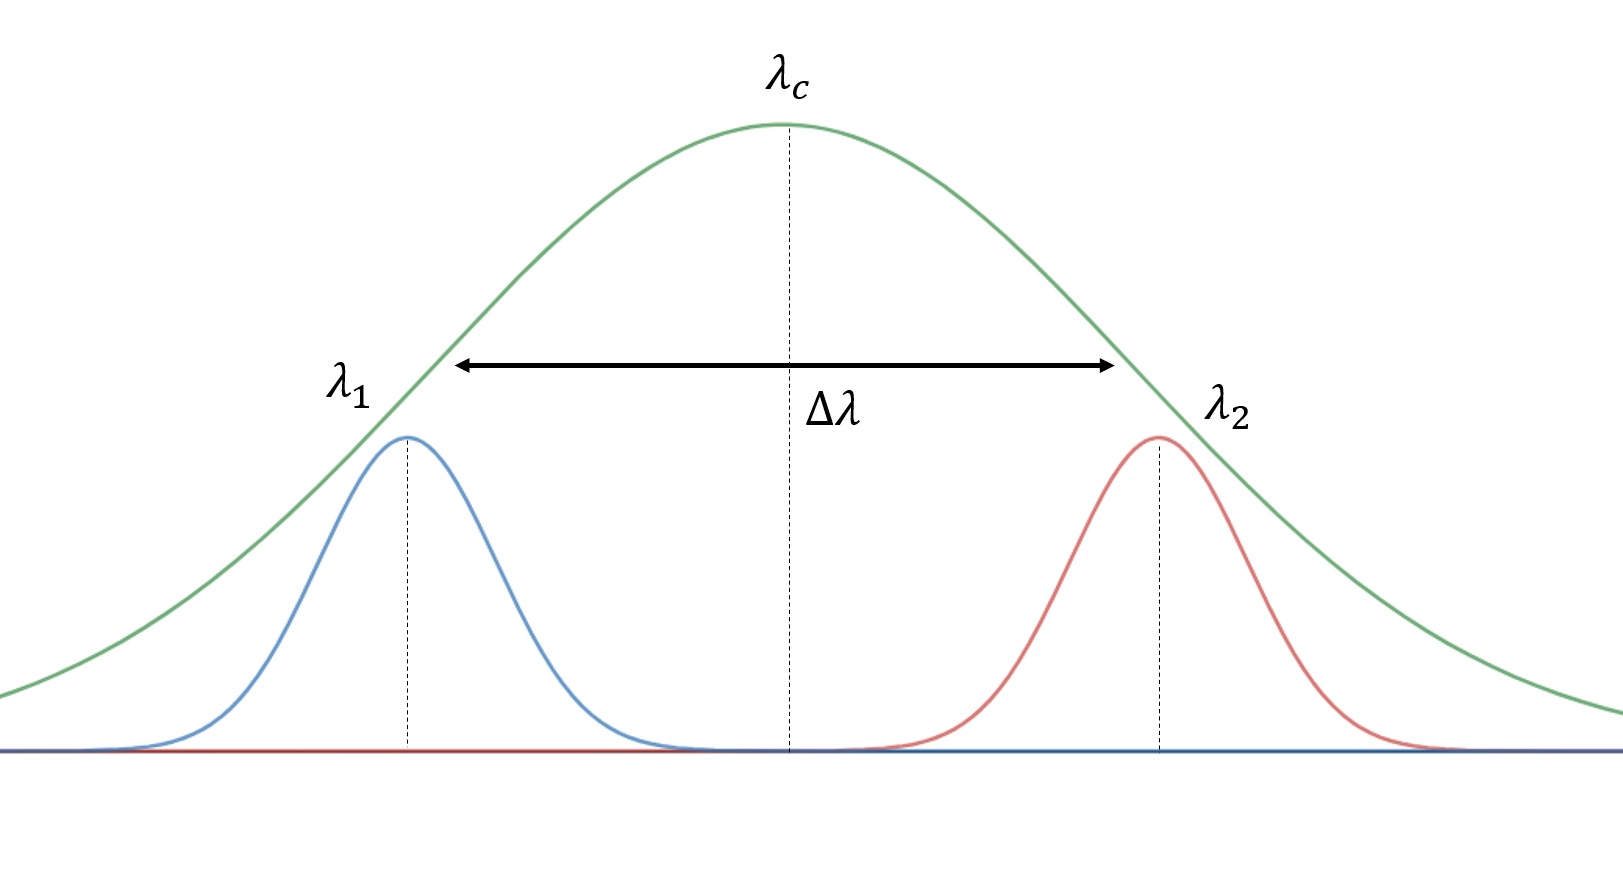
\includegraphics[width=\linewidth]{Figuras/GVD.png}
    \caption{Group velocity dispersion is proportional to the differences in group velocity at the ends of the pulse's spectral bandwidth.}
    \label{fig:GVD}
\end{figure}

Now we take the expression for the time difference and show that
\begin{align}
    \Delta\tau&=\frac{L}{c}\frac{dN_g}{d\lambda}\Delta\lambda\\
    &=\frac{L}{c}\frac{d}{d\lambda}\left(n-\lambda\frac{dn}{d\lambda}\right)\Delta\lambda\\
    &=-\frac{L}{c}\lambda\frac{d^2n}{d\lambda^2}\Delta\lambda.
\end{align}
And on that basis we define
\begin{equation}
    D\equiv-\frac{\lambda}{c}\frac{d^2n}{d\lambda^2}
\end{equation}
the \textbf{material dispersion}. Two things should be intuitively clear from these results:
\begin{enumerate}
    \item First, the fact that it depends on the second derivative of the refractive index with respect to wavelength. Knowing that group velocity itself is depend on such a derivative, and that group velocity dispersion is evaluated by comparing group velocities of adjacent carrier wavelengths, this is the only possible result. In other words, for group velocity we were asking about how the index changes as we move through the spectrum, for the material (group velocity) dispersion, we are asking how this ``change'' changes along the spectrum, it has ``second derivative'' written all over it.
    \item Second, that it describes a pulse broadening in time, which justifies is description as a \textbf{dispersion} term. This is a well-known result from quantum mechanics, where the dispersion relation derived from the Schrodinger equation will describe the broadening of the wave-function. In general, the physics of a system will determine a dispersion relation, which in turn will dictate the distinction between phase velocity and group velocity.
\end{enumerate}

\subsection{Modal dispersion}

Now we consider a second source of pulse spreading: the differences in the group velocities at which the allowed modes travel in a waveguide.

Consider a low-order mode: its wavevector is almost parallel to the $z$ axis, and therefore its propagation coefficient is very close to $\beta\approx k_0n_{core}$, so its effective index is also very similar to the core. Low-order modes are very easily guided, in the sense that its normalized effective index $b$ goes up from zero very quickly as the normalized frequency grows. Remember that the numerator in the $b$ parameter is proportional to the attenuation coefficient $\gamma$, so such low order modes are well-confined in the core, as is the case in general for modes away from cut-off. The lowest order mode is a special case only in the sense that it is almost always away from cutoff, as shown in Figure \ref{fig:characteric.equation}.

The high-order modes are easy to describe now. They correspond to wavevectors making a higher angle with the $z$ axis, therefore the propagation coefficient is smaller then $k_0n_{core}$. These modes are found more often near cut-off, where the attenuation coefficient is smaller, and the field is not so well-confined.

So instead of talking about high or low order modes, let us just talk about modes near and far from cut-off, while simply keeping in mind that the higher order your mode is, the higher your normalized frequency has to be in order to confine it well within your waveguide.

What is the point of all this discussion: 
\begin{itemize}
    \item Modes near cut-off travel effectively at the group velocity allowed by the cladding, precisely because that's where most of the field is.
    \item Modes away from cut-off travel effectively at the group velocity allowed by the core, because they are well confined.
\end{itemize}

All of this should be obvious just by looking at Figure \ref{fig:characteric.equation}, and reminding yourself that the attenuation coefficient grows with the normalized effective index\footnote{$\gamma$ and $b$ are not functions of each other in any meaningful physical sense, they just depend on some of the same parameters. For any given waveguide geometry, there is no way to increase $b$ without increasing the attenuation coefficient}. 

This is very different from material dispersion. In that case, we were talking about how the group velocities of spectral constituents of the pulse differ across its bandwidth, and cause it to spread as it propagates. Here, we are talking about how the boundary conditions of specific waveguide geometries force different modes to propagate in different media, since they are not equally confined in the core, therefore changing their group velocities. If the input energy of the optical pulse excites multiple modes, some of them will be more confined then others, and since your actual \textit{signal} (be it described in terms of energy or information) travels at the group velocity, it will be spread in time, much like in the case of material dispersion, but for an entirely different reason.

Now we need to find an expression for this time delay introduced between the modes. By analogy alone we could say that
\begin{equation}
    v_g=\frac{d\omega}{dk}\;\;\Rightarrow\;\;\tau_g=\frac{dk}{d\omega}\;\;\;\xRightarrow{waveguide}\;\;\;\tau_g=\frac{d\beta}{d\omega}.
\end{equation}
The full time delay (per unit length) will be given by the difference between the lowest and highest order modes. For the lowest, we write $\beta\approx k_0n_{core}$, and for the highest $\beta\approx k_0n_{cladding}$\footnote{Remember that $\beta=k_0n_1\sin{\theta_1}$, and that highest order modes are close the critical angle, for which $\sin{\theta_1}=n_2/n_1$. Another way to convince yourself of this approximation is to say that high order modes should have $n_{eff}$ close to the cladding value.}, therefore
\begin{equation}
    \tau_i=\frac{d\beta_i}{d\omega}=\frac{d}{d\omega}\left(\frac{n_i\omega}{c}\right)=\frac{n_i}{c}+k_0\frac{dn_i}{d\omega},
\end{equation}
and the difference is
\begin{equation}
    \Delta\tau_g=\frac{n_{core}-n_{cladding}}{c}+k_0\left(\frac{dn_{core}}{d\omega}-\frac{dn_{cladding}}{d\omega}\right).
\end{equation}
Note that even if there is no difference in the core/cladding material dispersion, there is still some dispersion due to differences in the effective $z$ components of the wavevector.

\subsection{Waveguide dispersion}

Before, we noted that group velocity in a medium depends on the derivative of $\omega$ with respect to $k$. Therefore, if an optical pulse has some spectral width, which will always be the case, we showed  that the discrepancy in group velocities arising from both ends of the spectral width will be proportional to the second derivative $\partial^2\omega/\partial k^2$, and that this will dictate group velocity dispersion.

Now, consider also that the spectral width in a single mode inside a waveguide is enough to bring different values of $\beta$ into the picture, even when discussing a single mode. In our discussion of modal dispersion, we noted that the time delay per unit length for a pulse in a waveguide is given by
\begin{equation}
    \tau_g=\frac{d\beta}{d\omega}\;\;\;\;\xRightarrow{intuition}\;\;\;\;D_{wd}\propto\frac{d^2\beta}{d\omega^2},
\end{equation}
so much like in the case of group velocity dispersion, we can predict that the so-called waveguide dispersion will be proportional to the second derivative of $\beta$ with respect to $\omega$. If the rate at which $\beta$ changes with $\omega$ predicts the group velocity for one spectral component of a pulse, than the rate at which this previous rate changes along the spectral width of a single mode is obviously responsible for the discrepancies between pulses that forms the physical basis for dispersion. The reason why changes in $\beta$ correspond to changes in the velocities is similar to the case we discussed for modal dispersion: the effective group index associated with each $k$ changes as the modes become more or less confined to the core.

We are now in a position to consider both \textit{material dispersion} and \textit{waveguide dispersion} as two forms of \textbf{chromatic and intra-modal dispersion} and \textit{modal dispersion} as a form of \textbf{intermodal dispersion}.

We know that results for the mode eigenvalue $\beta$ are found by solving a transcendental equation. We also know that this equation contains some wavelength dependence, via the wavevector $k$. In other words, the propagation constant $\beta$ has some strange wavelength dependence, so we should not expect to extract an analytical expression, instead we may write
\begin{equation}
    \Delta\tau_{wg}=\frac{1}{c}\left(\frac{d\beta_1}{dk}-\frac{d\beta_2}{dk}\right)\approx\frac{1}{c}\frac{d^2\beta}{dk^2}\Delta k,
\end{equation}
for a pulse with a spectral bandwidth $\Delta k$. In terms of wavelength, this is the same as
\begin{equation}
    \Delta\tau_{wg}=-\frac{k^2}{2\pi c}\frac{d^2\beta}{dk^2}\Delta\lambda.
\end{equation}
Waveguide dispersion is generally of a lower magnitude than material and modal dispersion. It does, however, become specially relevant for single mode systems operating near the point of zero material dispersion.

\subsection{Are material and waveguide dispersion the same?}

Many textbooks describe waveguide dispersion as being a case of ``material dispersion in a waveguide'', such that you only need to change the wavevector by the propagation constant in order to go from one to the other. Although this is mostly true mathematically, it is a misleading equivalence in any physical sense. What they have in common is that both are sources of \textbf{group velocity dispersion}, but the reasons why such dispersion appears are quite different in each case.

In the most general case, that of material dispersion, group velocity dispersion will depend on how the group velocity shifts along the bandwidth of an optical pulse, due to the spectral dependence of the refractive index. There are many acceptable ways of quantifying this dispersion,
\begin{align}
    \Delta\tau_g&=\frac{\partial \tau_g}{\partial \omega}\Delta\omega=\frac{\partial}{\partial \omega}\frac{1}{v_g}\Delta\omega=\frac{\partial^2k}{\partial\omega^2}\Delta\omega\;\;\;\Rightarrow\;\;\;[D]=\left[\frac{\partial^2k}{\partial\omega^2}\right]=\frac{s}{m\cdot\frac{rad}{s}}\\
    &=\frac{1}{c}\Delta N_g=\frac{1}{c}\frac{\partial N_g}{\partial \lambda}\Delta\lambda=-\frac{\lambda}{c}\frac{d^2n}{d\lambda^2}\Delta\lambda\;\;\;\Rightarrow\;\;\;[D]=\left[-\frac{\lambda}{c}\frac{d^2n}{d\lambda^2}\right]=\frac{s}{m\cdot m}
\end{align}
These two expressions are entirely equivalent. Both express an amount of delay per unit of distance per ``spectral'' unit (frequency or wavelength), indicating that the dispersion will be larger if the path is longer or if the bandwidth is larger.

The first expressions allows a more straight forward comparison with the waveguide dispersion case. The second, by making use of the effective group index, highlights the physical source of dispersion: the spectral dependence of refractive index.

In the less general case, that of waveguide dispersion, group velocity dispersion will also depend on how the group velocity shifts along the spectral bandwidth of the pulse, but now it is due to the spectral dependence of the allowed propagation coefficient, determined by the transcendental characteristic equation. The comparison to the general case is easy if you accept that it only makes sense to describe the group delay along the propagation direction of the waveguide, which is why we need only go from $k$ to $\beta$. In this case, we can write it as
\begin{equation}
    \Delta\tau_{wg}&=\frac{\partial \tau_{wg}}{\partial \omega}\Delta\omega=\frac{\partial}{\partial \omega}\frac{1}{v_{wg}}\Delta\omega=\frac{\partial^2\beta}{\partial\omega^2}\Delta\omega\;\;\;\Rightarrow\;\;\;[D]=\left[\frac{\partial^2\beta}{\partial\omega^2}\right]=\frac{s}{m\cdot\frac{rad}{s}}
\end{equation}

And once again, the units will tell the whole story. To conclude this chapter, let us see if we can identify the sources of dispersion in Figure \ref{fig:dispersion.diagram}. The use of normalized parameters would make measurements of dispersion much more complicated, so I will focus only on their meaning. The contribution to material dispersion comes simply from the fact there is a pulse of some width traveling in a medium with some spectral response. This same width will also correspond to some number of possible propagation coefficients, which lead to waveguide dispersion. The discrepancy in propagation coefficients in even larger across modes, and this variability will lead to modal dispersion.

\begin{figure}[H]
    \centering
    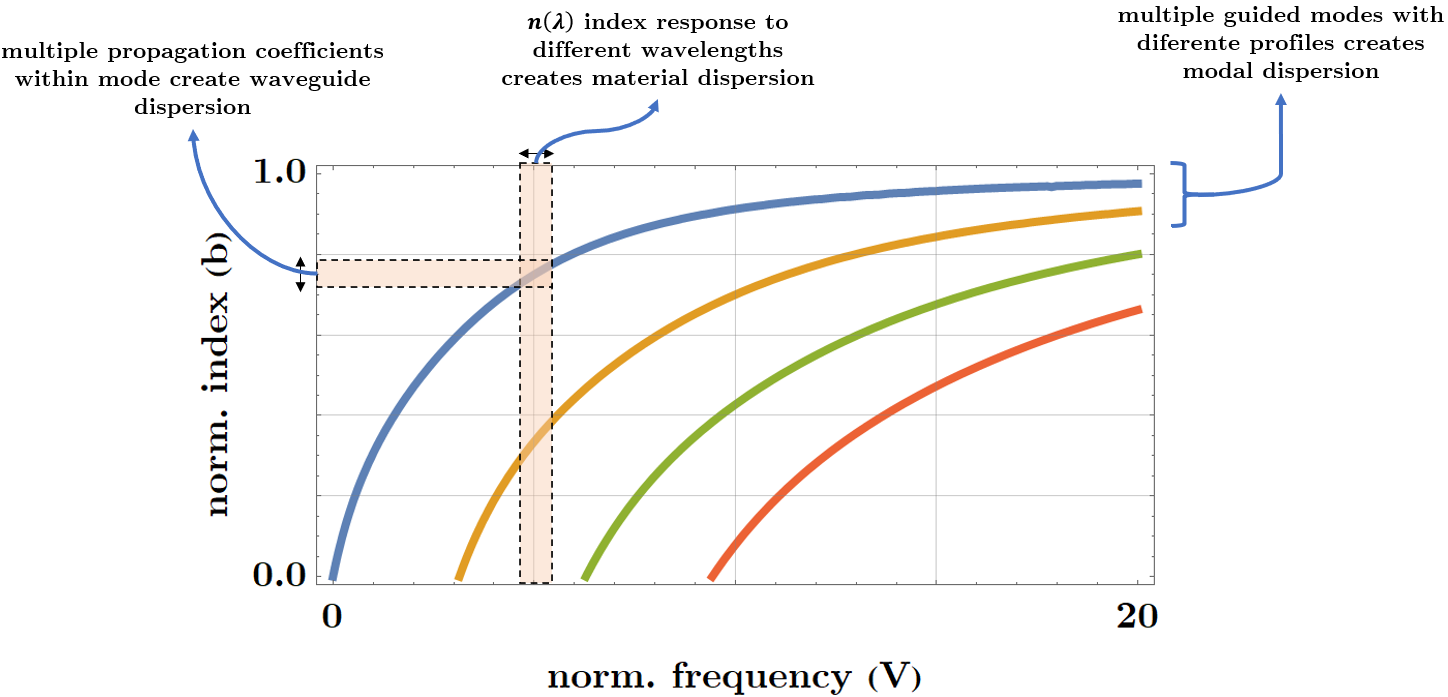
\includegraphics[width=1\linewidth]{Figuras/dispersion types diagram.png}
    \caption{Three contributions to dispersion in a waveguide (OBS consertar retângulo)}
    \label{fig:dispersion.diagram}
\end{figure}

\subsection{Why is it a second derivative?}

If you ever begin to question why these equations depend on a \textbf{second} derivative, look at Figure \ref{fig:GVD} again. When we talk about group velocity dispersion, we are talking about the spectral dependency of the group velocity, which is itself given by spectral dependency.

The first dependency appears because, when you are adding up multiple frequencies to form a pulse, you have to know how the $\omega/k$ ratios (phase velocities) will change along your bandwidth, because this will determine your group velocity. You do this by evaluating the derivative at the carrier frequency.

But if you have a Fourier sum of infinite frequencies, you can't just ignore the fact that \textbf{maybe these ratios change in different ways in different regions of the spectrum}, and if these changes are significant along the bandwidth of your pulse, than you will have group velocity dispersion. This is why the second derivative appears.

This should not be a surprise. We derived an expression for the group velocity based on a Taylor expansion for the dispersion relation $\omega(k)$, which neglected higher order terms by assuming the amplitudes were sharply peaked. Estimating the group velocity by evaluating the derivative at the carrier frequency was always an approximation, it is no surprise that the actual time delay introduced by GVD always appears multiplied by some sort of bandwidth: because this correction is only necessary where our initial approximation failed, and it only failed to the extent that the peak was not sharp enough!

Why is modal dispersion the only one that does not depend on a second derivative? Because in this case, we are not ``taking a closer look in the spectrum'', we are just taking into account the discreteness of the guided modes, and noting that if our initial pulse excited more than one of them, it never made any sense to treat them all with a single group velocity, given that their profiles are so different, regardless of how sharp the spectrum is.

\hrulefill

This concludes the review of optical waveguides.

\hrulefill




\chapter{Basic Concepts of Nonlinear Optics}

How do the symmetry properties of crystals give rise to optical susceptibility tensors.

\chapter{Nonlinear Interactions in Waveguides}

This is also an extremely important chapter. Modeling nonlinear interactions in waveguides is essential for running and interpreting simulations, and the results can be extended to more complicated systems like optical resonators and yields a convenient way to write quantized field equations.

\section{The Poynting theorem and mode orthogonality}

\noindent \textbf{obs.:} think of this section as a lemma. I am only trying to prove a result that will be important for a single step in the subsequent step\\

Normalization choices for fields in a guided mode depend heavily on the defintion of the poyting vector, whose most simple expression is a direct consequence of conservation of energy. Simply note that the  rate of work done by the fields is
%
\begin{equation}
\int_V \textbf{J}\cdot\textbf{E}\;\;d^3x=\int_V\left[\textbf{E}\cdot\left(\nabla\times\textbf{H}-\frac{\partial\textbf{D}}{\partial t}\right)\right]d^3x,
\end{equation}
%
Using the expression for the divergence of the cross product, we get
%
\begin{equation}
\textbf{E}\cdot(\nabla\times\textbf{H})-\textbf{E}\cdot\frac{\partial\textbf{D}}{\partial t}=-\nabla\cdot(\textbf{E}\times\textbf{H})+\textbf{H}\cdot(\nabla\times\textbf{E})-\textbf{E}\cdot\frac{\partial\textbf{D}}{\partial t}.
\end{equation}
%
Therefore
\begin{equation}
\int_V \textbf{J}\cdot\textbf{E}\;\;d^3x=-\int_V\left(\nabla\cdot(\textbf{E}\times\textbf{H})+\textbf{H}\cdot\frac{\partial\textbf{B}}{\partial t}+\textbf{E}\cdot\frac{\partial\textbf{D}}{\partial t}\right)d^3x.
\end{equation}

Now, if we were to neglect magnetization and polarization ($\chi_e=\chi_m=0$, $\epsilon=\epsilon_0$ and $\mu=\mu_0$) as well as dispersion and losses, we could write the total energy $u$ such that
\begin{equation}
u=\frac{1}{2}\left(\textbf{E}\cdot\textbf{D}+\textbf{B}\cdot\textbf{H}\right)\;\;\Rightarrow\;\;\int_V \textbf{J}\cdot\textbf{E}\;\;d^3x=-\int_V\left(\nabla\cdot(\textbf{E}\times\textbf{H})+\frac{\partial u}{\partial t}\right)d^3x.
\end{equation}

Which is where the Poynting vector would appear
%
\begin{equation}
\boxed{\textbf{S}\equiv\textbf{E}\times\textbf{H}\;\;\;\Rightarrow\;\;\;-(\textbf{J}\cdot\textbf{E})=\nabla\cdot\textbf{S}+\frac{\partial u}{\partial t}}.
\end{equation}

The complex Poynting vector, in turn, appears when we consider a quantity whose real part is the \textit{time-averaged} rate of work done by the fields in the volume. If the fields vary harmonically in time, we could write
%
\begin{align}
\textbf{J}(\textbf{r},t)\cdot\textbf{E}(\textbf{r},t)&=\frac{1}{4}\left[\left(\textbf{J}(\textbf{r})e^{-i\omega t}+\textbf{J}^*(\textbf{r})e^{i\omega t}\right)\times\left(\textbf{E}(\textbf{r})e^{-i\omega t}+\textbf{E}^*(\textbf{r})e^{i\omega t}\right)\right]\\
&=\frac{1}{2}\Re\left[\textbf{J}^*(\textbf{r})\cdot\textbf{E}(\textbf{r})+\textbf{J}(\textbf{r})\cdot\textbf{E}(\textbf{r})e^{-2i\omega t}\right].
\end{align}
%
When we take the time average of this quantity, the oscillating term will vanish, such that
%

\begin{equation}
    \Re\left[\frac{1}{2}\int_V \textbf{J}^*(\textbf{r})\cdot\textbf{E}(\textbf{r})\;d^3x\right]=\left\langle\frac{d}{dt}W\right\rangle.
\end{equation}

Now we follow the same procedure as before, but now using Maxwell's equations for harmonic time variation of the fields (I'll omit it, but there is only spatial dependence here),
%
\begin{align}
    \frac{1}{2}\int_V \textbf{J}^*\cdot\textbf{E}\;d^3x&=\frac{1}{2}\int_V\textbf{E}\cdot\left[\nabla\times\textbf{H}^*-i\omega\textbf{D}^*\right]d^3x\\
    &= \frac{1}{2}\int_V\left[-\nabla\cdot(\textbf{E}\times\textbf{H}^*)-i\omega(\textbf{E}\cdot\textbf{D}^*-\textbf{B}\cdot\textbf{H}^*)\right]
\end{align}.
%
Which motivates the definition of the complex Poynting vector
\begin{equation*}
    \textbf{S}=\frac{1}{2}\left[\textbf{E}(\textbf{r})\times\textbf{H}^*(\textbf{r})\right]
\end{equation*}

And the Poynting theorem for harmonic fields is written as
\begin{subequations}
\begin{equation}
    \frac{1}{2}\int_V\textbf{J}^*\cdot \textbf{E} \;d^3x+2i\omega\int_V(w_e-w_m)\;d^3x+\oint_S\textbf{S}\cdot\textbf{n}da=0
\end{equation}
\begin{equation}
    w_e=\frac{1}{4}(\textbf{E}\cdot\textbf{D}^*),\;\;\;\;w_m=\frac{1}{4}(\textbf{B}\cdot\textbf{H}^*)
\end{equation}
\end{subequations}
The real part of this equation gives the conservation of energy for the time-averaged quantities, and the imaginary part relates to the reactive or stored energy and its alternating flow.

This definition of the Poynting vector will be used to motivate our choice for normalization of fields in a waveguide. From Maxwell's Equations, consider two distinct guided modes $m$ and $n$
%
\begin{equation}
\begin{cases}
\nabla\times\textbf{E}_m^*=i\omega\mu_0\textbf{H}_m^*\\
\nabla\times\textbf{H}_m^*=-i\omega\epsilon_0\epsilon\textbf{E}_m^*\\
\nabla\times\textbf{E}_n=-i\omega\mu_0\textbf{H}_n\\
\nabla\times\textbf{H}_n=i\omega\epsilon_0\epsilon\textbf{E}_n
\end{cases}\;\;\;\Rightarrow\;\;\;
\begin{cases}
\textbf{H}_n\cdot(\nabla\times\textbf{E}_m^*)=i\omega\mu_0\textbf{H}_m^*\cdot\textbf{H}_n\\
\textbf{E}_n\cdot(\nabla\times\textbf{H}_m^*)=-i\omega\epsilon_0\epsilon\textbf{E}_m^*\cdot\textbf{E}_n\\
\textbf{H}_m^*\cdot(\nabla\times\textbf{E}_n)=-i\omega\mu_0\textbf{H}_n\cdot\textbf{H}_m^*\\
\textbf{E}_m^*\cdot(\nabla\times\textbf{H}_n)=i\omega\epsilon_0\epsilon\textbf{E}_n\cdot \textbf{E}_m^*
\end{cases}
\end{equation}
%
% \begin{gather}
%     \nabla\times\textbf{E}_m^*=i\omega\mu_0\textbf{H}_m^*\;\;\;\text{and}\;\;\;\nabla\times\textbf{H}_m^*=-i\omega\epsilon_0\epsilon\textbf{E}_m^*\\
%     \nabla\times\textbf{E}_n=-i\omega\mu_0\textbf{H}_n\;\;\;\text{and}\;\;\;\nabla\times\textbf{H}_n=i\omega\epsilon_0\epsilon\textbf{E}_n
% \end{gather}
%
% We may take the dot products, such that
% \begin{subequations}
% \begin{gather}
%     \textbf{H}_n\cdot\nabla\times\textbf{E}_m^*=i\omega\mu_0\textbf{H}_m^*\cdot\textbf{H}_n\;\;\;\text{and}\;\;\;\textbf{E}_n\cdot\nabla\times\textbf{H}_m^*=-i\omega\epsilon_0\epsilon\textbf{E}_m^*\cdot\textbf{E}_n\\
%     \textbf{H}_m^*\cdot\nabla\times\textbf{E}_n=-i\omega\mu_0\textbf{H}_n\cdot\textbf{H}_m^*\;\;\;\text{and}\;\;\;\textbf{E}_m^*\cdot\nabla\times\textbf{H}_n=i\omega\epsilon_0\epsilon\textbf{E}_n\cdot \textbf{E}_m^*
% \end{gather}
% \end{subequations}
%
%
Now we subtract the first and last equation:
%
\begin{equation}
    \textbf{H}_n\cdot(\nabla\times\textbf{E}_m^*)-\textbf{E}_m^*\cdot(\nabla\times\textbf{H}_n)=i\omega\mu_0\textbf{H}_m^*\cdot\textbf{H}_n-i\omega\epsilon_0\epsilon\textbf{E}_n\cdot \textbf{E}_m^*
\end{equation}
And the subtract the third by the second
%
\begin{equation}
    \textbf{H}_m^*\cdot(\nabla\times\textbf{E}_n)-\textbf{E}_n\cdot(\nabla\times\textbf{H}_m^*)=-i\omega\mu_0\textbf{H}_n\cdot\textbf{H}_m^*+i\omega\epsilon_0\epsilon\textbf{E}_m^*\cdot\textbf{E}_n
\end{equation}
%
And using the identity
\begin{equation}
    \nabla\cdot\left(\textbf{A}\times\textbf{B}\right)=(\nabla\times\textbf{A})\cdot\textbf{B}-(\nabla\times\textbf{B})\cdot\textbf{A}
\end{equation}
%
We demonstrate that
\begin{equation}
    \nabla\cdot\left(\textbf{E}_n\times\textbf{H}_m^*+\textbf{E}_m^*\times\textbf{H}_n\right)=0,
\end{equation}
which, for guided modes, can be rewritten as
\begin{equation}
    \left[\nabla_{(x,y)}+\frac{\partial}{\partial z}\right]\cdot\left(\textbf{E}_n(x,y)\times\textbf{H}^*_m(x,y)+\textbf{E}^*_m(x,y)\times\textbf{H}_n(x,y)\right)e^{-i(\beta_n-\beta_m)z}=0,
\end{equation}
therefore
\begin{multline}
    i(\beta_n-\beta_m)\left[\left(\textbf{E}_n(x,y)\times\textbf{H}^*_m(x,y)+\textbf{E}^*_m(x,y)\times\textbf{H}_n(x,y)\right)\cdot\hat{\textbf{z}}\right]=\\
    \nabla_{(x,y)}\cdot\left[\left(\textbf{E}_n(x,y)\times\textbf{H}^*_m(x,y)+\textbf{E}^*_m(x,y)\times\textbf{H}_n(x,y)\right)\right]_{(x,y)}
\end{multline}
Applying the divergence theorem in the plane, we may turn the right hand side into a line integral along an infinitely large contour on the xy plane. Since guided modes go to zero at infinity, the equation reduces to
\begin{equation}
    i(\beta_n-\beta_m)\iint\left[\left(\textbf{E}_n(x,y)\times\textbf{H}^*_m(x,y)+\textbf{E}^*_m(x,y)\times\textbf{H}_n(x,y)\right)\cdot\hat{\textbf{z}}\right]\;dx\,dy=0
\end{equation}
Therefore, when we consider two different modes, the integral must always vanish. However, for $m=n$, the integral has a particular meaning. Since
\begin{equation}
    \Re(z)=\frac{z+z^*}{2}
\end{equation}
then
\begin{multline}
    \iint\left[\left(\textbf{E}_m(x,y)\times\textbf{H}^*_m(x,y)+\textbf{E}^*_m(x,y)\times\textbf{H}_m(x,y)\right)\cdot\hat{\textbf{z}}\right]\;dx\,dy=\\2\Re\left[\iint\left[\textbf{E}_m(x,y)\times\textbf{H}^*_m(x,y)\right]\cdot\hat{\textbf{z}}\,dx\,dy\right]=2\Re\left[\iint\textbf{2S}\;dx\,dy\right]
\end{multline}
So we could write the \textbf{mode orthogonality condition} as
\begin{equation}
    \boxed{\iint\left[\left(\textbf{E}_n(x,y)\times\textbf{H}^*_m(x,y)+\textbf{E}^*_m(x,y)\times\textbf{H}_n(x,y)\right)\cdot\hat{\textbf{z}}\right]\;dx\,dy=4P_n\delta_{mn}},
\end{equation}
where $P_n$ is the mode power flow at the waveguide input. We can turn this into an \textbf{orthonormality} condition by normalizing the fields so as to have unit power flow.

In that case, we could define to vector quantities
\begin{equation}
    \textbf{F}_n(x, y, \omega) = \frac{1}{\sqrt{P_n(|\omega|)}}\textbf{E}_n(x, y, \omega) \;\;\;\text{and}\;\;\;\textbf{G}_n(x, y, \omega) = \frac{1}{\sqrt{P_n(|\omega|)}}\textbf{H}_n(x, y, \omega).
\end{equation}

which we might call the ``normalized mode profiles''.

\section{Perturbative Nonlinear Waveguide}

Now, instead of considering two modes $m$ and $n$, we consider first a mode propagating in a waveguide not exhibiting nonlinearity, and write it as
\begin{equation}
    \textbf{E}^{(0)}=\textbf{E}_m(x,y)\exp(-i\beta_mz)\;\;\;\text{and}\;\;\;\textbf{H}^{(0)}=\textbf{H}_m(x,y)\exp{-i\beta_mz}
    \label{eq:fields.definitions}
\end{equation}
ignoring the normalization for now. Additionally, we consider the guided modes
\begin{equation}
    \textbf{E}(\textbf{r})=\sum_mA_m(z,\omega)\textbf{E}_m(x,y)\exp{-i\beta_m z}\;\;\;\text{and}\;\;\;\textbf{H}(\textbf{r})=\sum_mA_m(z,\omega)\textbf{H}_m(x,y)\exp{-i\beta_m z}
\end{equation}
where the $A(z,\omega)$ is a dimensionless factor used to account for the $z$ dependence of the electric and magnetic fields, since we anticipate that the presence of the nonlinearity will cause different modes to become coupled.

The set of equations obeyed by these quantities is similar to the previous example, but now we add the polarization, such that
\begin{equation}
\begin{cases}
\nabla\times\textbf{E}^{(0)^*}=i\omega\mu_0\textbf{H}^{(0)^*}\\

\nabla\times\textbf{H}^{(0)^*}=-i\omega\epsilon_0\epsilon\textbf{E}^{(0)^*}\\

\nabla\times\textbf{E}=-i\omega\mu_0\textbf{H}\\

\nabla\times\textbf{H}=i\omega\left(\epsilon_0\epsilon\textbf{E}+\textbf{P}_{NL}\right)
\end{cases}\;\;\;\Rightarrow\;\;\;
%
\begin{cases}
\textbf{H}\cdot(\nabla\times\textbf{E}^{(0)^*})=i\omega\mu_0\textbf{H}^{(0)^*}\cdot\textbf{H}\\

\textbf{E}\cdot(\nabla\times\textbf{H}^{(0)^*})=-i\omega\epsilon_0\epsilon\textbf{E}^{(0)^*}\cdot\textbf{E}\\

\textbf{H}^{(0)}\cdot(\nabla\times\textbf{E})=-i\omega\mu_0\textbf{H}\cdot\textbf{H}^{(0)}\\

\textbf{E}^{(0)}\cdot(\nabla\times\textbf{H})=i\omega\left(\epsilon_0\epsilon\textbf{E}+\textbf{P}_{NL}\right)\cdot\textbf{E}^{(0)}
\end{cases}
\end{equation}

A quick comment is due on the $P_{NL}$ notation. Note that
\begin{equation}
    \textbf{D}=\varepsilon_0\textbf{E}+\textbf{P}=\varepsilon_0(1+\chi_e)\textbf{E}=\varepsilon_0\varepsilon\textbf{E}\;\;\text{s.t.}\;\;\;\textbf{P}=\varepsilon_0\left(\chi^{(1)}\textbf{E}(t)+\chi^{(2)}\textbf{E}^2(t)+\dots\right)
\end{equation}
which is to say that one may either write
\begin{equation}
    \textbf{D}=\varepsilon_0\textbf{E}+\textbf{P}\;\;\;\;\text{OR}\;\;\;\;\textbf{D}=\varepsilon_0\varepsilon\textbf{E}+\textbf{P}_{NL}
\end{equation}

And following the same procedure as before, we get to
\begin{equation}
    \nabla\cdot\left(\textbf{E}\times\textbf{H}^{(0)^*}+\textbf{E}^{(0)^*}\times\textbf{H}\right)=-i\omega\textbf{E}^{(0)^*}\cdot\textbf{P}_{NL}.
\end{equation}
Integrating this result in a volume parallel to the $xy$ plane with infinitely small thickness and infinite area, we get
\begin{equation}
    \iiint_V\nabla\cdot\left(\textbf{E}\times\textbf{H}^{(0)^*}+\textbf{E}^{(0)^*}\times\textbf{H}\right)\;dV=-i\omega\iiint_V\textbf{E}^{(0)^*}\cdot\textbf{P}_{NL}\;dV
\end{equation}
Separating the divergence in two terms,
\begin{multline*}
    \iiint_V\left[\nabla_{(x,y)}\cdot\left(\textbf{E}\times\textbf{H}^{(0)^*}+\textbf{E}^{(0)^*}\times\textbf{H}\right)_{(x,y)}\right]+\iiint_V\frac{\partial}{\partial z}\left(\textbf{E}\times\textbf{H}^{(0)^*}+\textbf{E}^{(0)^*}\times\textbf{H}\right)\cdot\hat{\textbf{z}}\;dV=\\
    =-i\omega\iiint_V\textbf{E}^{(0)^*}\cdot\textbf{P}_{NL}\;dV
\end{multline*}
And applying the divergence theorem to the integral containing the $(x,y)$ components,
\begin{multline*}
    \oiint_{\partial V}\left[\left(\textbf{E}\times\textbf{H}^{(0)^*}+\textbf{E}^{(0)^*}\times\textbf{H}\right)_{(x,y)}\right]\cdot d\textbf{S}+\iiint_V\frac{\partial}{\partial z}\left(\textbf{E}\times\textbf{H}^{(0)^*}+\textbf{E}^{(0)^*}\times\textbf{H}\right)\cdot\hat{\textbf{z}}\;dV=\\
    =-i\omega\iiint_V\textbf{E}^{(0)^*}\cdot\textbf{P}_{NL}\;dV
\end{multline*}
Since the guided modes go to zero at infinity, the first integral will vanish, for the same reason as before. And considering infinitely small thickness, we may rewrite the equation as
\begin{equation}
    \iint_S\frac{\partial}{\partial z}\left(\textbf{E}\times\textbf{H}^{(0)^*}+\textbf{E}^{(0)^*}\times\textbf{H}\right)\cdot\hat{\textbf{z}}\;dS  =-i\omega\iint_S\textbf{E}^{(0)^*}\cdot\textbf{P}_{NL}\;dS
\end{equation}
The only fields that will contribute to the cross product so as not to get a zero projection on $\hat{\textbf{z}}$ will be transverse, so
\begin{equation}
    \iint_S\frac{\partial}{\partial z}\left(\textbf{E}_T\times\textbf{H}_T^{(0)^*}+\textbf{E}_T^{(0)^*}\times\textbf{H}_T\right)\cdot\hat{\textbf{z}}\;dS  =-i\omega\iint_S\textbf{E}^{(0)^*}\cdot\textbf{P}_{NL}\;dS
\end{equation}
Notice that $T$ subscript is just a short notation for the $(x,y)$ argument. And by substituting the definitions of the fields, denoting the non-perturbed mode by $n$ and the perturbed mode by $m$, 
\begin{multline}
    \sum_m\frac{\partial}{\partial z}\left(A_m(z,\omega)e^{-i(\beta_m-\beta_n)z}\iint\left[\left(\textbf{E}_{T,m}\times\textbf{H}^*_{T,n}+\textbf{E}^*_{T,n}\times\textbf{H}_{T,m}\right)\cdot\hat{\textbf{z}}\right]\;dx\,dy\right)=\\=-i\omega\iint_S\textbf{E}_{m}^*(x,y)e^{i\beta_mz}\cdot\textbf{P}_{NL}\;dS
\end{multline}
and using the mode orthogonality condition, all terms in the summation will vanish, except for when $m=n$,
\begin{equation}
    \boxed{\frac{\partial}{\partial z} A_m(z,\omega)=-\frac{i\omega}{4P_m}e^{i\beta_mz}\iint_S\textbf{E}_{m}^*(x,y,\omega)\cdot\textbf{P}_{NL}(x,y,\omega)\;dx\,dy}
    \label{eq:overlap integral}
\end{equation}

Note that $A_m(z,\omega)$ describes the coupling between modes in a waveguide due to a nonlinear interaction, and that it is proportional to the \textbf{spatial overlap integral} between the unperturbed field and the nonlinear polarization vector.

% THIS IS A LARGE SECTION ON SECTION HARMONIC GENERATION, WHICH WAS READY BUT I DECIDED TO DO IT AGAIN BECAUSE THERE WAS A MISTAKE SOMEWHERE THAT I COULD NOT FIND FOR THE LIFE OF ME

% \section{Second Harmonic Generation}

% In order to provide a thorough description of SHG, we must first tackle two topics: (1) how to model waveguide grating employed in order to achieve quasi-phase matching, and (2) some notation on the nonlinear susceptibility tensor.

% \subsubsection{Waveguide grating}

% %\todo[inline]{To do: understand precisely why and when birefringence and other methods cease to work as a mechanism for phase-matching.}

% We can achieve any modulation of the relative permittivity through a Fourier series
% %
% \begin{equation}
%     \Delta\mtens{\epsilon}=\sum_q\Delta\mtens{\epsilon}_q(x,y)\exp\left(-i\frac{2\pi}{\Lambda}qz\right)
% \end{equation}
% %
% and similarly for the nonlinear susceptibility tensor $\mtens{d}=\chi(2\omega,\omega,\omega)$,
% %
% \begin{equation}
%     \Delta\mtens{d}=\sum_q\Delta\mtens{d}_q(x,y)\exp\left(-i\frac{2\pi}{\Lambda}qz\right)
% \end{equation}
% %
% \subsubsection{Nonlinear susceptibility tensor}

% When the fundamental input field, at frequency $\omega$ is incident in a nonlinear material, the second order polarization $\textbf{P}^{(2)}$ will include components of frequency $2\omega$ (second-harmonic generation) and zero (optical rectification). Therefore, in such a situation, there exist electric fields and polarizations of frequencies $\omega$ and $2\omega$ in the medium. In the time domain, we might therefore write
% %
% \begin{subequations}
% \begin{gather}
%     \textbf{E}(t)=\Re{\textbf{E}^{\omega}\exp(i\omega t)+\textbf{E}^{2\omega}\exp(i2\omega t)}\\
%     \textbf{P}(t)=\Re{\textbf{P}^{\omega}\exp(i\omega t)+\textbf{P}^{2\omega}\exp(i2\omega t)}
% \end{gather}
% \end{subequations}
% % 
% The linear polarizations are functions of the relative permittivity (I'll simply use bold face instead of tensor notation) and the input field
% %
% \begin{subequations}
% \begin{gather}
%     \textbf{P}_{(L)}^{\omega}=\epsilon_0 \Delta \bm{\epsilon}^{\omega}\textbf{E}^{\omega}\\
%     \textbf{P}_{(L)}^{2\omega}=\epsilon_0 \Delta \bm{\epsilon}^{2\omega}\textbf{E}^{2\omega}
% \end{gather}
% \end{subequations}

% For the non linear polarizatoin, we employ the following definition

% \begin{equation}
%     P_i^{(2)}(\omega)=\epsilon_0\chi^{(2)}_{ijk}(\omega)E_j(\omega')E_k(\omega-\omega')
% \end{equation}
% %
% which can be made equivalent to the following integral, just by considering the continuous analog $\chi^{(2)}_{ijk}\equiv\Tilde{\chi}^{(2)}_{ijk}\Delta\omega$, such that
% \begin{equation}
%     P^{(2)}_i(\omega)=\epsilon_0\int_{-\infty}^{\infty}d\omega'\Tilde{\chi}^{(2)}_{ijk}(\omega;\omega',\omega-\omega')E_j(\omega')E_k(\omega-\omega')
% \end{equation}
% %
% and therefore
% \begin{subequations}
% \begin{gather}
%     \textbf{P}_{(NL)}^{\omega}=2\epsilon_0\bm{d}\cdot\textbf{E}^{\bm{\omega}^*}\textbf{E}^{2\bm{\omega}}\\
%     \textbf{P}_{(NL)}^{2\bm{\omega}}=\epsilon_0\bm{d}\cdot\textbf{E}^{\bm{\omega}}\textbf{E}^{\bm{\omega}}
% \end{gather}
% \end{subequations}

% \subsubsection{Coupled Mode Equations for SHG}

% Now we must plug in all this results into the overlap integral derived in the previous section
% \begin{equation}
%     \frac{\partial}{\partial z}A_m(z)=-\frac{i\omega}{4P_m}\iint_S\textbf{E}^*_m(x,y,\omega)\cdot\textbf{P}(x,y,\omega)e^{i\beta_mz}\;dxdy
% \end{equation}
% For the input, $\omega$ frequency component, the equation becomes
% \begin{equation}
%     \frac{\partial A^{\omega}}{\partial z}=-\frac{i\omega}{4P_z^{\omega}}\iint_S\left[\textbf{E}^{\omega^*}(x,y)e^{i\beta^{\omega}z}\cdot\left(\epsilon_0\Delta\bm{\epsilon}^{\omega}\textbf{E}^{\omega}+2\epsilon_0\textbf{d}\textbf{E}^{\omega^*}\textbf{E}^{2\omega}\right)\right]dxdy
% \end{equation}
% \begin{multline}
%     \frac{\partial A^{\omega}}{\partial z}=-\frac{i\omega}{4P_z^{\omega}}\epsilon_0\iint_S\left[\Delta\bm{\epsilon}^{\omega}\textbf{E}^{\omega^*}(x,y)\cdot\textbf{E}^{\omega}(x,y)A^{\omega}(z)e^{-i(\beta^{\omega}-\beta^{\omega})z}+\\+2\textbf{d}\textbf{E}^{\omega^*}(x,y)\left[A^{\omega}(z)\right]^*A^{2\omega}(z)\textbf{E}^{\omega^*}(x,y)\textbf{E}^{2\omega}(x,y)e^{-i(\beta^{2\omega}-2\beta^{\omega})z}\right]dxdy
% \end{multline}
% \begin{multline}
%     \frac{\partial A^{\omega}}{\partial z}=-\frac{i\omega}{4P_z^{\omega}}\epsilon_0\iint_S\left(\left[\textbf{E}^{\omega}(x,y)\right]^*\cdot\left[\textbf{E}^{\omega}(x,y)\right]A^{\omega}(z)\sum_q\Delta\bm{\epsilon}(x,y)e^{-iKz}\right)dxdy+\\-\frac{i\omega}{4P_z^{\omega}}\epsilon_0\iint_S\left(\sum_q2\textbf{d}(x,y)\left[\textbf{E}^{\omega^{*}}\right]^*\left[A^{\omega}(z)\right]^*A^{2\omega}(z)\textbf{E}^{2\omega}(z)e^{-i(\beta^{2\omega}-2\beta^{\omega}-qK)z}\right)dxdy
% \end{multline}
% By selecting only the $q=\pm1$ terms so as to make the permittivity a cosine function, we come to
% \begin{equation}
% \frac{d}{dz}A^{\omega}(z)+i\left(2\kappa_L^\omega\cos(Kz)A^{\omega}(z)\right)=-i\sum_q\left[\kappa_{NL}^{(q)}\right]^*\exp(-i2\Delta_qz)\left[A^{\omega}(z)\right]^*A^{2\omega}(z)
% \end{equation}
% Where
% \begin{subequations}
% \begin{equation}
%     \kappa_L^{\omega}=\frac{\omega\epsilon_0}{4}\iint\left[E^{\omega}(x,y)\right]^*\Delta\bm{\epsilon}_1^{\omega}(x,y)\textbf{E}^{\omega}(x,y)\;dxdy\\
% \end{equation}
% \begin{equation}
%     \kappa_{NL}^{(q)}=\frac{2\omega\epsilon_0}{4}\iint\left[\textbf{E}^{2\omega}(x,y)\right]^*\textbf{d}_q(x,y)\left[\textbf{E}^{\omega}(x,y)\right]^2\;dxdy
% \end{equation}
% \end{subequations}

% And in order to obtain an equation for the $2\omega$ component, we need to go back and substitute a different polarization into the overlap integral. The resulting equation for $A^{2\omega}(z)$ is
% %
% \begin{equation}
%     \frac{d}{dz}A^{2\omega}(z)+i\left(2\kappa_L^{2\omega}\cos(Kz)A^{2\omega}(z)\right)=-i\sum_q\left[\kappa_{NL}^{(q)}\right]\exp(i2\Delta_qz)\left[A^{\omega}(z)\right]^2,
% \end{equation}
% where
% \begin{equation}
%     \kappa_{L}^{2\omega}=\frac{2\omega\epsilon_0}{4}\iint\left[E^{2\omega}(x,y)\right]^*\Delta\bm{\epsilon}_1^{2\omega}(x,y)\textbf{E}^{2\omega}(x,y)\;dxdy\\
% \end{equation}

% The coupled equations now predict that the amplitudes of the mode will change as the fields propagate in the $z$ direction in some manner proportional to the spatial overlap of the different fields. Coming back to the coupled equations
% \begin{subequations}
% \begin{equation}
%     \frac{d}{dz}A^{\omega}(z)+i\left(2\kappa_L^\omega\cos(Kz)A^{\omega}(z)\right)=-i\sum_q\left[\kappa_{NL}^{(q)}\right]^*\exp(-i2\Delta_qz)\left[A^{\omega}(z)\right]^*A^{2\omega}(z)
% \end{equation}
% \begin{equation}
%     \frac{d}{dz}A^{2\omega}(z)+i\left(2\kappa_L^{2\omega}\cos(Kz)A^{2\omega}(z)\right)=-i\sum_q\left[\kappa_{NL}^{(q)}\right]\exp(i2\Delta_qz)\left[A^{\omega}(z)\right]^2,
% \end{equation}
% \end{subequations}

% If we write
% \begin{subequations}
% \begin{gather}
%     A^{\omega}(z)=A(z)\exp\left(-i\frac{2\kappa_L^{\omega}}{K}\sin(Kz)\right)\\
%     A^{2\omega}(z)=B(z)\exp\left(-i\frac{2\kappa_L^{2\omega}}{K}\sin(Kz)\right)
% \end{gather}
% \end{subequations}
% %
% then
% %
% \begin{subequations*}
% \begin{gather*}
%     \frac{dA^{\omega}(z)}{dz}=\frac{dA(z)}{dz}\exp\left(-i\frac{2\kappa_L^{\omega}}{K}\sin(Kz)\right)-2iA(z)\kappa_L^{\omega}\cos(Kz)\exp\left(-i\frac{2\kappa_L^{\omega}}{K}\sin(Kz)\right)\\
%     \frac{A^{2\omega}(z)}{dz}=\frac{dB(z)}{dz}\exp\left(-i\frac{2\kappa_L^{2\omega}}{K}\sin(Kz)\right)-2iA(z)\kappa_L^{2\omega}\cos(Kz)\exp\left(-i\frac{2\kappa_L^{2\omega}}{K}\sin(Kz)\right)
% \end{gather*}
% \end{subequations*}
% %
% which is extremely useful, since it will cancel out the second term in each of the coupled equations. Once we divide both sides by the exponentials, we will end up with
% \begin{subequations}
% \begin{multline*}
%     \frac{d}{dz}A(z)-2iA(z)\kappa_L^{\omega}\cos(Kz)+i\left(2\kappa_L^\omega\cos(Kz)A(z)\right)=\\=-i\sum_q\left[\kappa_{NL}^{(q)}\right]^*\exp(-i2\Delta_qz)A^*(z)\exp\left(2i\frac{2\kappa_L^{\omega}}{K}\sin(Kz)\right)B(z)\exp\left(-i\frac{2\kappa_L^{2\omega}}{K}\sin(Kz)\right)
% \end{multline*}
% \begin{multline*}
%     \frac{d}{dz}B(z)-2iA(z)\kappa_L^{2\omega}\cos(Kz)+i\left(2\kappa_L^{2\omega}\cos(Kz)A^{2\omega}(z)\right)=\\=-i\sum_q\left[\kappa_{NL}^{(q)}\right]\exp(i2\Delta_qz)A^2(z)\exp\left(-2i\frac{2\kappa_L^{\omega}}{K}\sin(Kz)\right)\exp\left(i\frac{2\kappa_L^{2\omega}}{K}\sin(Kz)\right)\\
% \end{multline*}
% \end{subequations}
% and
% \begin{subequations}
% \begin{equation*}
%     \frac{d}{dz}A(z)=-i\sum_q\left[\kappa_{NL}^{(q)}\right]^*\exp(-i2\Delta_qz)A^*(z)\exp\left(2i\frac{2\kappa_L^{\omega}}{K}\sin(Kz)\right)B(z)\exp\left(-i\frac{2\kappa_L^{2\omega}}{K}\sin(Kz)\right)
% \end{equation*}
% \begin{equation*}
%     \frac{d}{dz}B(z)=-i\sum_q\left[\kappa_{NL}^{(q)}\right]\exp(i2\Delta_qz)A^2(z)\exp\left(-2i\frac{2\kappa_L^{\omega}}{K}\sin(Kz)\right)\exp\left(i\frac{2\kappa_L^{2\omega}}{K}\sin(Kz)\right)\\
% \end{equation*}
% \end{subequations}
% joining the exponentials
% \begin{subequations}
% \begin{equation*}
%     \frac{d}{dz}A(z)=-i\sum_q\left[\kappa_{NL}^{(q)}\right]^*\exp(-i2\Delta_qz)A^*(z)B(z)\exp\left(-i\left[\frac{2(\kappa_L^{2\omega}-2\kappa_L^{\omega})}{K}\right]\sin(Kz)\right)
    
%     %\exp\left(2i\frac{2\kappa_L^{\omega}}{K}\sin(Kz)\right)\exp\left(-i\frac{2\kappa_L^{2\omega}}{K}\sin(Kz)\right)
% \end{equation*}
% \begin{equation*}
%     \frac{d}{dz}B(z)=-i\sum_q\left[\kappa_{NL}^{(q)}\right]\exp(i2\Delta_qz)A^2(z)\exp\left(i\left[\frac{2(\kappa_L^{2\omega}-2\kappa_L^{\omega})}{K}\right]\sin(Kz)\right)
%     %\exp\left(-2i\frac{2\kappa_L^{\omega}}{K}\sin(Kz)\right)\\
% \end{equation*}
% \end{subequations}
% Therefore
% \begin{subequations}
% \begin{gather}
%     \frac{d}{dz}A(z)=-i\kappa^*A^*(z)B(z)\exp\left[-i(2\Delta)z\right]\\
%     \frac{d}{dz}B(z)=-i\kappa\left[A(z)\right]^2\exp\left[i(2\Delta)z\right]
% \end{gather}
% \end{subequations}

\section{Second Harmonic Generation}

Let us now consider the case of a very simple nonlinear process, in which a beam is incident upon a second order nonlinear crystal, and is converted to a signal of twice its frequency. The input (pump) field is given by
\begin{equation}
    \textbf{E}(\textbf{r})=A_p(z,\omega)\textbf{E}_p(x,y)\exp{-i\beta_m z}
    \label{eq:field}
\end{equation}
%
And the polarization is given by a tensor product, whose components can be written, in Einstein notation, as
\begin{equation}
    P^{(NL)}_i=\varepsilon_0\left(\chi^{(1)}_{ij}E_j+\chi^{(2)}_{ijk}E_jE_k+\chi^{(3)}_{ijkl}E_jE_kE_l\right)
\end{equation}
Notice that in obtaining Equation \ref{eq:overlap integral}, the first (linear) term was excluded from $\textbf{P}_{NL}$ via the relative electric permittivity $\varepsilon$. Additionally, let us assume we are dealing with a material exhibiting a large $\chi^{(2)}$ compared to its $\chi^{(3)}$ susceptibility. So
\begin{equation}
    \textbf{P}_{NL}=\varepsilon_0\Tilde{\chi}^{(2)}\textbf{E}^2
\end{equation}
Writing out each component, and now making the summations explicit
\begin{equation}
    P^{(NL)}_i(\omega_m+\omega_n)=\varepsilon_0\sum_{jk}\sum_{(nm)}2d_{ijk}E_j(\omega_n)E_k(\omega_m),\;\;\text{where}\;\;d_{ijk}=\frac{1}{2}\chi_{ijk}^{(2)}
\end{equation}
In order to best represent this in two dimensions, we will make the following assumptions
\begin{itemize}
    \item That there is symmetry in the exchange of the last two indices (jk), such that the following substitutions may take place
    \begin{equation*}
       \text{jk}\rightarrow\text{l}:\;\;11\rightarrow1,\;\;22\rightarrow2,\;\;33\rightarrow3,\;\;23,32\rightarrow4,\;\;13,31\rightarrow5,\;\;12,21\rightarrow6
    \end{equation*}
    This assumption is valid in the presence of Kleinman's symmetry, and also valid in general for SHG, since $\omega_m=\omega_n$. The susceptibility can now be written as
    \begin{equation*}
        d_{il}=\begin{pmatrix}
            d_{11} & d_{12} & d_{13} & d_{14} & d_{15} & d_{16}\\
            d_{21} & d_{22} & d_{23} & d_{24} & d_{25} & d_{26}\\
            d_{31} & d_{32} & d_{33} & d_{34} & d_{35} & d_{36}
        \end{pmatrix}
    \end{equation*}
    \item That Kleinman's symmetry is valid, such that all indexes can be permuted freely, such that many terms cease to be independent
    \begin{equation*}
        d_{12}=d_{122}=d_{212}=d_{26},\;\;\;d_{14}=d_{123}=d_{213}=d_{25},\;\;\;\text{and so on...}
    \end{equation*}
    \begin{equation*}
        d_{il}=\begin{pmatrix}
            d_{11} & d_{12} & d_{13} & d_{14} & d_{15} & d_{16}\\
            d_{16} & d_{22} & d_{23} & d_{24} & d_{14} & d_{12}\\
            d_{15} & d_{24} & d_{33} & d_{23} & d_{13} & d_{14}
        \end{pmatrix}
    \end{equation*}
\end{itemize}
Now the final expression for the nonlinear polarization is
\begin{equation}
\begin{pmatrix}
    P^{(NL)}_x(\omega_1+\omega_2) \\P^{(NL)}_y(\omega_1+\omega_2)\\P^{(NL)}_z(\omega_1+\omega_2)\end{pmatrix}=4\varepsilon_0
    \begin{pmatrix}
        d_{11} & d_{12} & d_{13} & d_{14} & d_{15} & d_{16}\\
        d_{16} & d_{22} & d_{23} & d_{24} & d_{14} & d_{12}\\
        d_{15} & d_{24} & d_{33} & d_{23} & d_{13} & d_{14}
    \end{pmatrix}\begin{pmatrix}
        E_x(\omega_1)E_x(\omega_2)\\
        E_y(\omega_1)E_y(\omega_2)\\
        E_z(\omega_1)E_z(\omega_1)\\
        E_y(\omega_1)E_z(\omega_2)+E_z(\omega_1)E_y(\omega_2)\\
        E_x(\omega_1)E_z(\omega_2)+E_z(\omega_1)E_x(\omega_2)\\
        E_x(\omega_1)E_y(\omega_2)+E_y(\omega_1)+E_x(\omega_2)
    \end{pmatrix}
\end{equation}
And even more simply, for second harmonic generation we'll have
\begin{equation}
\begin{pmatrix}
    P^{(NL)}_x(2\omega) \\P^{(NL)}_y(2\omega)\\P^{(NL)}_z(2\omega)\end{pmatrix}=2\varepsilon_0
    \begin{pmatrix}
        d_{11} & d_{12} & d_{13} & d_{14} & d_{15} & d_{16}\\
        d_{16} & d_{22} & d_{23} & d_{24} & d_{14} & d_{12}\\
        d_{15} & d_{24} & d_{33} & d_{23} & d_{13} & d_{14}
    \end{pmatrix}\begin{pmatrix}
        E_x(\omega)^2\\
        E_y(\omega)^2\\
        E_z(\omega)^2\\
        2E_y(\omega)E_z(\omega)\\
        2E_x(\omega)E_z(\omega)\\
        2E_x(\omega)E_y(\omega)
    \end{pmatrix}
\end{equation}
But now consider a waveguide-like system where a z-cut nonlinear crystal like Lithium Niobate displays a very large optical nonlinearity along its z-axis ($d_{33} = 27 pm/V$), such that all other contributions are negligible in comparison to it.

We generally have $z$ point in the propagation direction of the waveguide, but now notice that a $z-cut$ crystal will have its z-axis point upwards towards the cladding (either $x$ or $y$ in the original reference frame). So a quasi-TM mode (or a TM mode in a slab waveguide), whose electric field is best aligned with the $z$ direction, will mostly likely display optimal nonlinear coupling in such a system. In this case we can write
\begin{equation}
    \textbf{P}^{(NL)}=2\varepsilon_0d_{\text{eff}}E^2(\omega)\hat{\textbf{z}}=2\varepsilon_0d_{33}E^2_z(\omega)\hat{\textbf{z}},
\end{equation}
recovering the definition in Equation \ref{eq:field}, we get
\begin{equation}
    \textbf{P}^{(NL)}=2\varepsilon_0 d_{33}A^2(z,\omega)E^2_\omega(x,y)\exp{-2i\beta^\omega z}\hat{\textbf{z}}
\end{equation}
Plugging this result back into the integral from \ref{eq:overlap integral}
\begin{equation}
    \frac{\partial}{\partial z} A_m(z,\omega)=-\frac{i\omega}{4P_m}e^{i\beta_mz}\iint_S\textbf{E}_{m}^*(x,y,\omega)\cdot\textbf{P}_{NL}(x,y,\omega)\;dx\,dy
\end{equation}
\begin{multline}
    \frac{\partial}{\partial z} A^{2\omega}(z)=-\frac{i\omega}{4P_m}\exp{i\beta^{2\omega} z}\iint_S\left[E^{2\omega}(x,y)\hat{\textbf{z}}\right]^*\cdot\\\cdot\left[2\varepsilon_0 d_{33}\left(A^{\omega}(z,\omega)E^\omega(x,y)\right)^2\exp{-2i\beta^\omega z}\hat{\textbf{z}}\right]\;dx\,dy
\end{multline}
notice that the $\textbf{E}^*_m(x,y,\omega)$ factor does not contain its own $z$ dependent amplitude. It was included in the ``perturbative waveguide solution'' precisely by virtue of representing the unperturbed mode, which differs from the perturbed mode by the presence of the $A(z,\omega)$ factor. Additionally, its $z$-dependent \textit{factor} is already written explicitly, and taken outside the integral.
\begin{equation}
    \frac{\partial}{\partial z} A^{2\omega}(z)=-\frac{i\omega}{4P_m}\left[A^{\omega}(z)\right]^2e^{i(\beta^{2\omega}-2\beta^{\omega}) z}\iint_S\left[E^{2\omega}(x,y)\right]^*\left[2\varepsilon_0 d_{33}\left(E^\omega(x,y)\right)^2\right]\;dx\,dy
\end{equation}
All the variables in this equation could have been written with a $m$ subscript, given that it holds true for any of the multiple modes corresponding to the frequencies involved. The final result could be written as
\begin{equation}
    \begin{cases}
        \frac{\partial}{\partial z} A^{2\omega}(z)=-i\kappa\left(\frac{\omega\varepsilon_0d_{33}}{2P_m}\right)\left[A^{\omega}(z)\right]^2e^{i(\beta^{2\omega}-2\beta^{\omega}) z}\\
        \kappa=\iint_S\left[E^{2\omega}(x,y)\right]^*\left[E^\omega(x,y)\right]^2\;dx\,dy
    \end{cases}
\end{equation}
this is a good place to stop for a quick unit check. Equation \ref{eq:fields.definitions} ensures that $A(z,\omega)$ must be dimensionless, so the left-hand-side has units determined by the spatial derivative alone, so
\begin{equation*}
    \frac{1}{m}=-i\left[\iint_S\left[E^{2\omega}(x,y)\right]^*\left[E_\omega(x,y)\right]^2\;dx\,dy\right]\left[\frac{\omega\varepsilon_0d_{33}}{2P_m}\right]\left[A^{\omega}(z)^2e^{i(\beta^{2\omega}-2\beta^{\omega}) z}\right]\\
\end{equation*}
\begin{equation*}
    \frac{1}{m}=\left(\frac{V^3}{m^3}\right)m^2\frac{\frac{1}{s}\cdot\frac{F}{m}\cdot\frac{m}{V}}{W}=
    \left(\frac{V^3}{m}\right)\frac{\frac{1}{s}\cdot \frac{C}{V}\cdot\frac{1}{V}}{W}=\frac{V\cdot C}{s\cdot m \cdot W}=\frac{J\cdot C}{C\cdot s\cdot m\cdot W}=\frac{1}{m}
\end{equation*}
this indicates that the result checks out. An interesting point is to look at the solution under a no-pump depletion approximation, that is, $A^\omega(z)=A_0$, such that under an integration from $0<z<L$
\begin{equation}
    A(L)=-\frac{i\kappa\omega\varepsilon_0d_{33}A_0^2}{2P_m}\left(\frac{e^{i\Delta\beta L}-1}{i\Delta}\right)=-\frac{i\kappa\omega\varepsilon_0d_{33}A_0^2}{P_m}\left(e^{i\Delta\beta L}\right)\frac{\sin{\left(\frac{1}{2}\Delta\beta L\right)}}{\frac{1}{2}\Delta\beta L}
\end{equation}
\begin{equation}
    A(L)=-\frac{i\kappa\omega\varepsilon_0d_{33}A_0^2}{P_m}\left(e^{i\Delta\beta L}\right)\text{sinc}{\left(\frac{1}{2}\Delta\beta L\right)}
\end{equation}
this result clearly highlights the importance of the phase matching condition. Notice that $\Delta\beta=\beta^{2\omega}-2\beta^{\omega}$ should be zero for efficiency to be optimal, which is equivalent to requiring that the propagation constant be linear relative to frequency (in other words, requiring net zero velocity dispersion).

\section{Sum Frequency Generation}

Page 56 Suhara

\section{Parametric Down Conversion}

\chapter{Optical Cavities}

Consider a simple Fabry-Perot resonator consisting of three mirrors, of which only one is responsible for coupling light in and out of the resonator, as in Figure \ref{fig:fabry.perot}. The field can be written as a function of the position along the internal cavity path, ranging form $0$ to $L$. Our goal is to study the interaction between these fields, and how they relate to the properties of the resonator.

\begin{figure}[H]
    \centering
    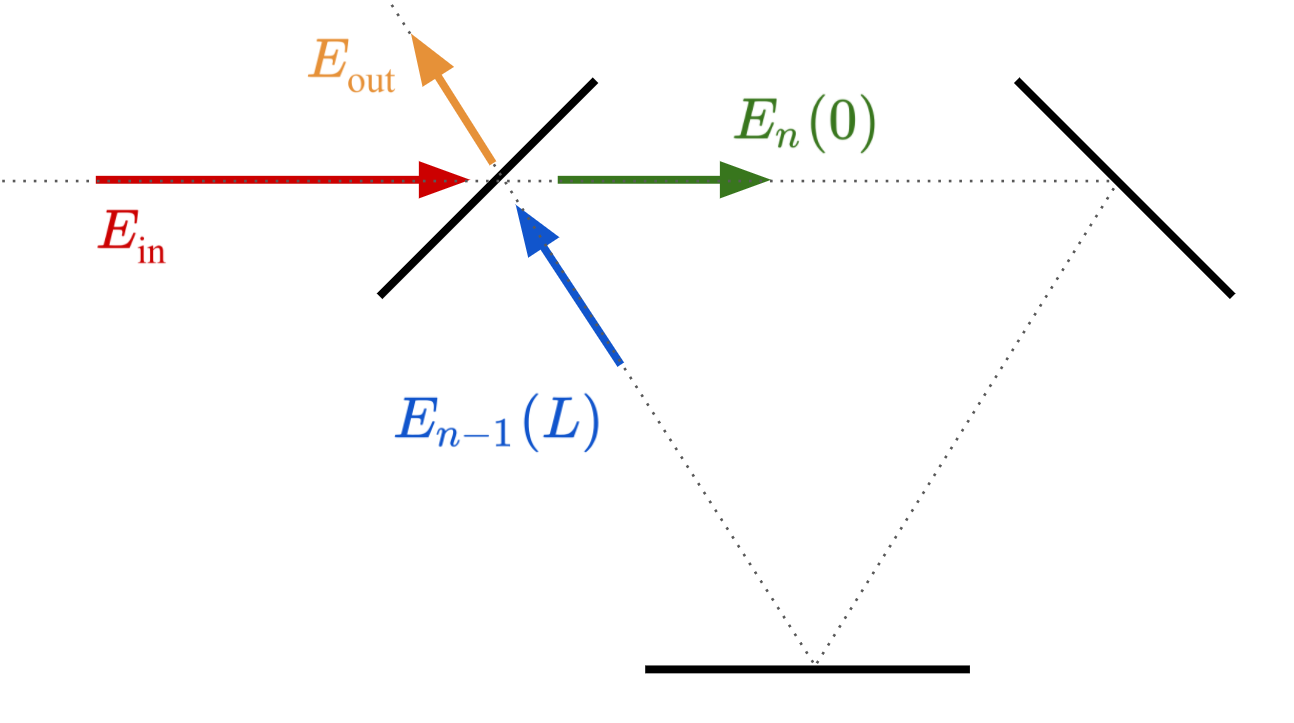
\includegraphics[width=0.75\linewidth]{Figuras/fabry-perot model.png}
    \caption{Fabry-perot resonator.}
    \label{fig:fabry.perot}
\end{figure}

This result will be demonstrated in such a  way as to make it easily generalizable to more complex systems. In that sense, the inside of the cavity can be treated as a ``black box'' containing only one port where the light can couple in and out, and inside of which the field gains some phase and undergoes some loss (with few adjustments it can also exhibit nonlinear effects).

We begin by writing a simple beam-splitter equation for the fields described in Figure \ref{fig:fabry.perot}, that is
%
\begin{equation}
    \begin{cases}
    E_{out}=\sqrt{T}E_{n-1}(L)-\sqrt{R}E_{in}\\[0.5cm]
    E_{n}(0)=\sqrt{R}E_{n-1}(L)+\sqrt{T}E_{in}
    \end{cases}
    \label{eq:beam splitter}
\end{equation}
%
and the goal is to write the change in the electric field between two consecutive round-trips
%
\begin{equation}
    \Delta E = E_n(0)-E_{n-1}(0)
\end{equation}
for each trip, we assume the field must undergo a phase shift proportional to its propagation constant $\beta(\omega)$. Additionally, losses can be modeled as an exponential decay along the length $L$ of the cavity, determined by an ``attenuation coefficient'' $\alpha$. Finally, losses due to imperfect reflection by the intra-cavity mirrors can be summarized by a reflection coefficient $\sqrt{R_b}$ (distinct from the coefficient $\sqrt{R}$ at the coupling mirror), then
%
\begin{equation}
    E_{n-1}(L)=\exp{i\beta(\omega)L}\exp{-\frac{\alpha}{2}L}\sqrt{R_b}E_{n-1}(0)
\end{equation}
Notice that the $1/2$ factor in the exponent of the attenuation term is convenient when we switch to a description in terms of energy rather than amplitude, since the former is proportional to the square of the latter. The function $\beta(\omega)$ in the phase shift term can be expanded as a Taylor series around the resonance frequency $\omega_0$ and the detuning $\delta\omega=\omega-\omega_0$, such that
\begin{equation}
    \exp{i\beta(\omega)L}=\exp(i\beta(\omega_0)L)\exp(i\beta^{(1)}\delta\omega L)\dots
\end{equation}
%
where I have only kept terms up to first order in $\delta\omega$. The first term is equal to one by the definition of the \textit{resonance} frequency. The resonance frequency of a Fabry-Perot cavity is precisely one in which the field will accumulate a $\phi=2\pi$ phase-shift at each round trip, thus $\beta(\omega_0)L=2\pi$. We are now left with
%
\begin{equation}
    E_{n-1}(L)=\exp(i\beta^{(1)}\delta\omega L)\exp(-\frac{\alpha}{2}L)\sqrt{R_b}E_{n-1}(0).
\end{equation}
Ignoring higher order terms in $i\delta\omega L$ (near-resonance operation), $\alpha L$ (low attenuation) and $T_b$ (high reflectance of the intra-cavity mirrors), the expression becomes
\begin{equation}
    E_{n-1}(L)=(1+i\beta^{(1)}\delta\omega L)\left(1-\frac{\alpha L}{2}\right)\left(1-\frac{T_b}{2}\right)E_{n-1}(0)
\end{equation}
where we have used the general relation $\sqrt{R}=\sqrt{1-T}$. Carrying out the multiplication we get to
\begin{equation*}
    E_{n-1}(L)=\left(1-\frac{\alpha L}{2}+i\beta^{(1)}\delta\omega L - \frac{1}{2}i\beta^{(1)}\delta\omega L^2\alpha\right)\left(1-\frac{T_b}{2}\right)E_{n-1}(0),
\end{equation*}
discarding the last term in the first parenthesis
\begin{equation*}
    E_{n-1}(L)=\left(1-\frac{\alpha L}{2}+i\beta^{(1)}\delta\omega L\right)\left(1-\frac{T_b}{2}\right)E_{n-1}(0),
\end{equation*}
\begin{equation*}
    E_{n-1}(L)=\left(1-\frac{T_b}{2}-\frac{\alpha L}{2}+\frac{1}{4}\alpha L T_b+i\beta^{(1)}\delta\omega L-i\beta^{(1)}\delta\omega L\frac{T_b}{2}\right)E_{n-1}(0)
\end{equation*}
Finally, ignoring the other second-order terms,
\begin{equation}
    E_{n-1}(L)=\left(1+i\beta^{(1)}\delta\omega L - \frac{1}{2}(T_b+\alpha L)\right)E_{n-1}(0).
\end{equation}
Now, going back to the beam-splitter equation above,
\begin{equation}
    \begin{aligned}
        E_n(0)&=\sqrt{R}E_{n-1}(L)+\sqrt{T}E_{in}\\
        &=\left(1-\frac{T}{2}\right)\left(1+i\beta^{(1)}\delta\omega L - \frac{1}{2}(T_b+\alpha L)\right)E_{n-1}(0)+\sqrt{T}E_{in}\\
        &\approx\left(1+i\beta^{(1)}\delta\omega L - \frac{1}{2}(T+T_b+\alpha L)\right)E_{n-1}(0)+\sqrt{T}E_{in}
    \end{aligned}    
\end{equation}
we get to a position where we can finally write the change in the electric field between two consecutive round-trips
\begin{equation}
    \begin{aligned}
        \Delta E&=E_n(0)-E_{n-1}(0)\\
        &=\left(1+i\beta^{(1)}\delta\omega L - \frac{1}{2}(T+T_b+\alpha L)\right)E_{n-1}(0)+\sqrt{T}E_{in}-E_{n-1}(0)\\
        &=\left(i\beta^{(1)}\delta\omega L - \frac{1}{2}(T+T_b+\alpha L)\right)E_{n-1}(0)+\sqrt{T}E_{in}\\
        &\equiv \left(i\beta^{(1)}\delta L-\frac{\gamma}{2}\right)E_{n-1}(0)+\sqrt{T}E_{in}
    \end{aligned}    
\end{equation}
where I have defined $\gamma=(T+T_b+\alpha L)/2$ and $\delta\omega=\delta$ for simplicity. If we divide the whole equation by $t_R=L/v_g=L\beta^{(1)}$, we get to
\begin{equation}
    \frac{\Delta E}{t_R}=\left(i\delta-\frac{\gamma}{2t_R}\right)E_{n-1}(0)+\frac{\sqrt{T}}{\sqrt{t_R}}\frac{E_{in}}{\sqrt{t_R}}.
\end{equation}
Notice now that the energy density inside the cavity is such that
\begin{equation}
    U\propto |E|^2\;\;\;\Rightarrow\;\;\;U=c|E|^2=\hbar\omega\Bar{n}\equiv\hbar\omega|\alpha|^2,
\end{equation}
which allows us to write a correspondence between the field $E$ and the dimensionless quantity $\alpha$ related to the average number of photons
\begin{equation}
    E=\frac{\hbar\omega}{C}\alpha=\frac{1}{K}\alpha.
\end{equation}
So in order for the whole equation to be in terms of $E$, we should multiply it all by the constant $K$
\begin{equation}
    K\frac{\Delta E}{t_R}=\left(i\delta-\frac{\gamma}{2t_R}\right)KE_{n-1}(0)+\frac{\sqrt{T}}{\sqrt{t_R}}K\frac{E_{in}}{\sqrt{t_R}}.
\end{equation}
Finally, we take the limit where the number of round-trips is infinite, such that $t_R\rightarrow 0$ and all the field terms become alpha terms. Once we make
\begin{equation}
    \sqrt{\gamma_{in}}=\frac{\sqrt{T}}{\sqrt{t_R}}\;\;\;\text{and}\;\;\;\alpha_{in}=\lim_{n\rightarrow\infty}\left(K\frac{E_{in}}{\sqrt{t_R}}\right)\;\;\text{such that}\;\;|\alpha_{in}|^2=\frac{\Bar{n}}{t_R}
\end{equation}
Thus, the final expression for the Fabry Perot equation is
\begin{equation}
    \boxed{\frac{d\alpha}{dt}=\left(i\delta-\frac{\gamma}{2}\right)\alpha+\sqrt{\gamma_{in}}\alpha_{in}}
    \label{eq:final.fabry.perot}
\end{equation}

\subsection*{Steady-state operation}
Consider the case where the resonator is operating at a steady state, such that the derivative in Equation \ref{eq:final.fabry.perot} is zero
\begin{equation}
    \frac{d\alpha}{dt}=0\;\;\;\Rightarrow \alpha=\frac{\sqrt{\gamma_{in}}\alpha_{in}}{\left(\frac{\gamma}{2}-i\delta\right)}
\end{equation}
We should hold on to that result for a second, and take a look at what can be said about the cavity's emission. Equation \ref{eq:beam splitter} told us that
\begin{equation}
    E_{out}=\sqrt{T}E_{n-1}(L)-\sqrt{R}E_{in}
\end{equation}
when operating at the steady state, we can safely approximate $E_{n-1}(L)\approx E_{n-1}(0)$. Then, by multiplying for $K$, dividing by $\sqrt{t_R}$ and taking the limit, we come back to the $\alpha$ notation
\begin{equation}
    \alpha_{out}=\sqrt{\gamma_{in}}\alpha-\alpha_{in}
    \label{eq:output.fabry.perot}
\end{equation}
where $\alpha_{out}$ \textbf{has been defined so as to have units of $1/\sqrt{t}$, and have its square be equivalent to mean outward photon flux, exactly like $\alpha_{in}$}. In turn, $\gamma_{in}$ is exactly like the one defined previously.

Now we can throw the steady-state field result from equation \ref{eq:final.fabry.perot} into equation \ref{eq:output.fabry.perot}, such that
\begin{equation}
    \alpha_{out}=\alpha_{in}\left(\frac{\gamma_{in}}{\frac{\gamma}{2}-i\delta}-1\right).
\end{equation}
Now we are able to define e general \textbf{reflection coefficient} for the whole Fabry-Perot cavity
\begin{equation}
    R_{FB}=\left|\frac{\alpha_{out}}{\alpha_{in}}\right|^2=\left|1+\frac{\gamma_{in}}{i\delta-\frac{\gamma}{2}}\right|^2
\end{equation}
where I have multiplied by $-1$ inside the modulus and flipped the signs in the denominator to make things tidier. To add physical intuition, let us separate the components of the terms relating to loss
\begin{equation}
    \gamma_{in}=\frac{T}{t_R}\;\;\;\;\;\gamma=\frac{T+T_b+\alpha L}{t_R}\equiv \gamma_{in}+\mu
\end{equation}
By this definition, $\mu$ becomes a term containing only \textbf{intracavity losses} (which dissipate energy from the incoming light), and $\gamma_{in}$ contains only the \textbf{coupling losses} (which divert incoming energy outwards, and still contribute to cavity emission).

We can rewrite the cavity reflection coefficient as
\begin{equation}
    R_{FB}=\left|\frac{\alpha_{out}}{\alpha_{in}}\right|^2=\left|1+\frac{\gamma_{in}}{i\delta-\frac{\gamma_{in}+\mu}{2}}\right|^2.
\end{equation}
And plot it as in Figure \ref{fig:reflectance.plot}.

\begin{figure}[H]
    \centering
    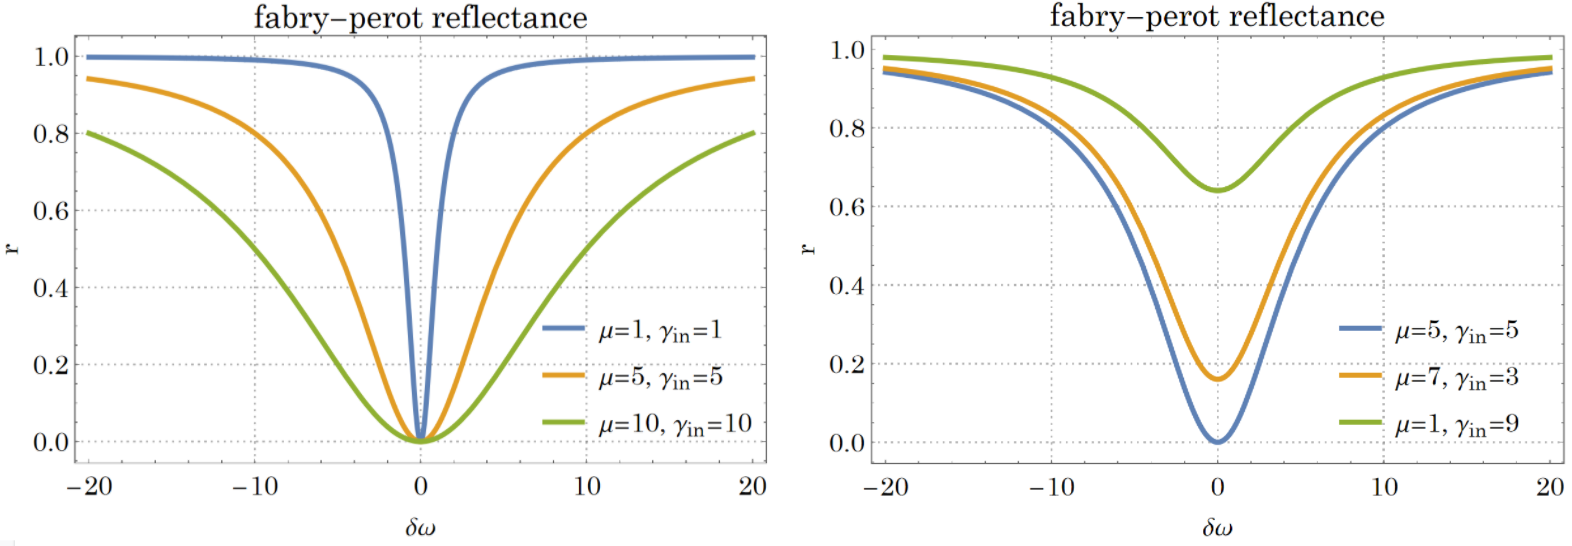
\includegraphics[width=1\linewidth]{Figuras/fabry-perot reflectance plot.png}
    \caption{Reflectance of a Fabry-Perot interferometer. In the first plot, varying the magnitude of both contributions to loss. In the second plot, varying their difference.}
    \label{fig:reflectance.plot}
\end{figure}

Surprisingly enough, if we simplify the complex modulus, we can rewrite once again as
\begin{equation}
    R_{FB}=1-\frac{\mu\gamma_{in}}{\delta^2+\frac{1}{4}(\gamma_{in}+\mu)^2},
\end{equation}
which makes the contributions from internal losses and coupling losses interchangeable. Since the peak always occurs at $\delta=0$, it is easy to demonstrate that the ``depth'' of the peak is always given by
\begin{equation}
    R_{min}=1-\frac{\mu\gamma_{in}}{\frac{1}{4}(\gamma_{in}+\mu)^2}=\frac{(\gamma_{in}-\mu)^2}{(\gamma_{in}+\mu)^2}=\left(\frac{\gamma_{in}-\mu}{\gamma}\right)^2.
\end{equation}
And the width, being the $\delta\omega$ value at which half of $R_{min}$ is reached is easily obtained from the previous result






\chapter{Classical Theory of the Optical Parametric Oscillator}
phD Felippe página 35

\chapter{Basic Concepts of Quantum Optics}

\chapter{Squeezing}

\printbibliography





\end{document}